\documentclass[a4paper,12pt]{book}
\usepackage{graphicx}
\usepackage{float}
\usepackage[hidelinks]{hyperref}
\usepackage{subcaption}
\usepackage{dirtree}
\usepackage{etoolbox}
\usepackage{booktabs}
\apptocmd{\dirtree}{\bigskip}{}{}
\pretocmd{\dirtree}{\bigskip}{}{}
\graphicspath{ {./images/} }

\hypersetup{
	colorlinks,
	linkcolor=red,
	urlcolor=blue}

%opening
\title{Warsaw scanning report}
\author{Miłosz Wojciechowski}
\date{\today}

\begin{document}


\maketitle
\pagebreak
\tableofcontents
\pagebreak

\chapter{Introduction}
This document serves as a report of Mandeye (documentation available \href{https://github.com/JanuszBedkowski/mandeye_controller/tree/main/doc/manual/manual_v0_2}{here}) scanning process and creating a 3D model of a part of Warsaw. Project  included 4 phases:

\begin{itemize}
	\item planning
	\item field scanning using Mandeye scanner
	\item fixing trajectories and aligning scans (using \href{https://github.com/MapsHD/HDMapping}{HDMapping software})
	\item synchronizing scans with with \href{https://isok.gov.pl/index.html}{ISOK LIDAR data} downloaded for free from \href{URL}{geoportal}
\end{itemize}

For every scan its planned route, covered route and date is be provided. Scans were performed using \href{https://github.com/JanuszBedkowski/mandeye_controller/tree/main}{Mandeye mobile scanning system}. Routes were planned and visualized in QGIS (\url{https://qgis.org/pl/site/index.html}) using database \href{BDOT10k}{https://www.geoportal.gov.pl/pl/dane/baza-danych-obiektow-topograficznych-bdot10k/} and covered routes where registered by a GoPro MAX camera and its GNSS module. Telemetry data and frames were extracted using
\href{https://github.com/miloszwojciechowski/Warsaw-model/tree/main/GoPro-Telemetry-Extractor}{GoPro telemetry extractor} and \href{https://github.com/miloszwojciechowski/Warsaw-model/tree/main/GoPro_MAX_video_parser}{GoPro MAX video parser}. Interval between extracted frames is 3 seconds.\\

\pagebreak

\section{File structure}
File structure: 
\dirtree{%
.1 continousScanning-XXXX.
.2 GoPro.
.3 GSXXXXXX\_frames.
.4 jpg files.
.3 GSXXXXXX recording files.
.3 GSXXXXXX\_GPS file.
.3 GSXXXXXX\_telemetry file.
.2 preview.
.3 laz files.
.2 Mandeye scanner output files and files created by HDMapping.
}

\begin{itemize}
	\item \verb|continousScanning_XXXX| folder - major scan folder, XXXX stands for scan number e.g. 0001
	\item GoPro folder - for GoPro data (extracted frames, recording files, GPS.csv file and telemetry.csv file)
	\item \verb|GSXXXXXX_frames| folder - contains all extracted frames, in jpg format with 3 seconds interval between every frame
	\item GSXXXXXX recording files - these are 3 output files generated by a GoPro MAX camera - .360, .LRV and .THM. To get more information about them read \href{https://github.com/miloszwojciechowski/Warsaw-model/tree/main/Manuals/GoPro_MAX_video_parser}{GoPro MAX video parser manual}. XXXXXX stands for video number, given by the GoPro camera e.g. GS010100
	\pagebreak
	\item \verb|GSXXXXXX_GPS file| - csv file containing telemetry data extended by additional 2 columns (cts and images). Full name scheme is: \verb|GSXXXXXX_GPS_Interval_Value| where  XXXXXX stands for video number given by the GoPro camera e.g. GS010101, Interval equals either Frames or Seconds (depends which one was used to extract frames in \href{https://github.com/miloszwojciechowski/Warsaw-model/tree/main/GoPro_MAX_video_parser}{GoPro MAX video parser}) and Value is a number of Frames or Seconds which had to pass to extract another frame. All scans except for the \verb|continousScanning_0000| have \verb|GS010101_GPS_6_Frames.csv| file. Structure is described below:
	\begin{enumerate}
		\item Column without a name, index column created during video processing
		\item Date: year-month-day T hour:minute:second.millisecond Z
		\item Timestamp: in milliseconds
		\item Latitude: in degrees in WGS84
		\item Longitude: in degrees in WGS84
		\item Altitude: in meters
		\item Cts: timestamp calculated from Date column, in milliseconds
		\item Images: paths to frames located in a computer memory
	\end{enumerate}
	\item \verb|GSXXXXXX_telemetry file| - csv file containing telemetry data.  XXXXXX stands for video number, given by the GoPro camera e.g. GS010102. Structure described below:
	\begin{enumerate}
		\item Date: year-month-day T hour:minute:second.millisecond Z
		\item Timestamp: in milliseconds
		\item Latitude: in degrees in WGS84
		\item Longitude: in degrees in WGS84
		\item Altitude: in meters
	\end{enumerate}
\end{itemize}


\section{Scanning schedule}
\begin{figure}[H]
	\centering
	\includegraphics[width=1\linewidth]{Routes}
	\caption{All scanning routes.}
\end{figure}

\begin{figure}[H]
	\centering
	\includegraphics[width=1\linewidth]{Scan_zones}
	\caption{Areas covered by scans.}
\end{figure}
% Table generated by Excel2LaTeX from sheet 'Arkusz1'
\begin{table}[htbp]
  \centering
  \caption{Scan routes schedule.}
    \resizebox{\textwidth}{!}{\begin{tabular}{|c|c|c|c|c|}
    \toprule
    Route ID & Scan folder name & Planned length[km] & Covered length[km] & Data \\
    \midrule
    \hyperref[fig:fig0]{0}     & continousScanning\_0000 & 6,97  & 7,12  & 13.09.2023 \\
    \midrule
    \hyperref[fig:fig1]{1}     & continousScanning\_0001 & 9,65  & 9,46  & 14.09.2023 \\
    \midrule
    \hyperref[fig:fig2]{2}     & continousScanning\_0002 & 6,48  & 6,59  & 18.09.2023 \\
    \midrule
    \hyperref[fig:fig3]{3}     & continousScanning\_0003 & 4,82  & 5,85  & 19.09.2023 \\
    \midrule
    \hyperref[fig:fig4]{4}     & continousScanning\_0004 & 5,06  & 4,99  & 20.09.2023 \\
    \midrule
    \hyperref[fig:fig5]{5}     & continousScanning\_0005 & 5,78  & 6,44  & 21.09.2023 \\
    \midrule
    \hyperref[fig:fig6]{6}     & continousScanning\_0006 & 5,65  & 6,11  & 22.09.2023 \\
    \midrule
    \hyperref[fig:fig7]{7}     & continousScanning\_0007 & 5,77  & 7,38  & 25.09.2023 \\
    \midrule
    \hyperref[fig:fig8]{8}     & continousScanning\_0008 & 6,61  & 6,89  & 26.09.2023 \\
    \midrule
    \hyperref[fig:fig9]{9}     & continousScanning\_0009 & 5,34  & 5,82  & 27.09.2023 \\
    \midrule
    \hyperref[fig:fig10]{10}    & continousScanning\_0010 & 6,46  & 6,91  & 28.09.2023 \\
    \midrule
    \hyperref[fig:fig11]{11}    & continousScanning\_0011 & 4,62  & 4,85  & 29.09.2023 \\
    \midrule
    \hyperref[fig:fig12]{12}    & continousScanning\_0012 & 6,23  & 6,65  & 02.10.2023 \\
    \midrule
    \hyperref[fig:fig13]{13}    & continousScanning\_0013 & 4,72  & 5,45  & 03.10.2023 \\
    \midrule
    \hyperref[fig:fig14]{14}    & continousScanning\_0014 & 5,09  & 5,58  & 04.10.2023 \\
    \midrule
    \hyperref[fig:fig15]{15}    & continousScanning\_0015 & 5,07  & 6,3   & 05.10.2023 \\
    \midrule
    \hyperref[fig:fig16]{16}    & continousScanning\_0016 & 6,57  & 6,89  & 06.10.2023 \\
    \midrule
    \hyperref[fig:fig17]{17}    & continousScanning\_0017 & 5,60  & 7,06  & 09.10.2023 \\
    \midrule
    -     & -     & \multicolumn{2}{c|}{A week break caused by my absence} & \multicolumn{1}{l|}{10.10-16.10} \\
    \midrule
    \hyperref[fig:fig18]{18}    & continousScanning\_0018 & 4,80  & 5,47  & 17.10.2023 \\
    \midrule
    \hyperref[fig:fig19]{19}    & continousScanning\_0019 & 4,56  & 5,05  & 18.10.2023 \\
    \midrule
    \hyperref[fig:fig20]{20}    & continousScanning\_0020 & 5,34  & 5,54  & 19.10.2023 \\
    \midrule
    \hyperref[fig:fig21]{21}    & continousScanning\_0021 & 5,54  & 6,15  & 20.10.2023 \\
    \midrule
    \hyperref[fig:fig22]{22}    & continousScanning\_0022 & 4,73  & 4,88  & 23.10.2023 \\
    \midrule
    \hyperref[fig:fig23]{23}    & continousScanning\_0023 & 5,23  & 6,43  & 24.10.2023 \\
    \midrule
    -     & -     & \multicolumn{2}{c|}{Postponed due to rainfall} & 25.10.2023 \\
    \midrule
    \hyperref[fig:fig24]{24}    & continousScanning\_0024 & 5,34  & 5,57  & 26.10.2023 \\
    \midrule
    \hyperref[fig:fig25]{25}    & continousScanning\_0025 & 5,27  & 6,4   & 27.10.2023 \\
    \midrule
    \hyperref[fig:fig26]{26}    & continousScanning\_0026 & 5,12  & 5,75  & 30.10.2023 \\
    \midrule
    -     & -     & \multicolumn{2}{c|}{Postponed due to rainfall} & 31.10.2023 \\
    \midrule
    \hyperref[fig:fig27]{27}    & continousScanning\_0027 & 6,03  & 6,42  & 02.11.2023 \\
    \midrule
    \hyperref[fig:fig28]{28}    & continousScanning\_0028 & 5,49  & 6,88  & 03.11.2023 \\
    \midrule
    \hyperref[fig:fig29]{29}    & continousScanning\_0029 & 7,06  & 7,85  & 06.11.2023 \\
    \bottomrule
    \end{tabular}}%
  \label{tab:addlabel}%
\end{table}%



\chapter{Scans}
\section{Week 11-15 September 2023}
Scans conducted: continousScanning\_0000|, continousScanning\_0001.\\

It was a week with first scans and served as a test of how should it be done. Two scans were conducted - on Wednesday and Thursday.
\begin{enumerate}
	\item \textbf{13.09.2023} Scan 0000. \\
	 Wednesday scan focused on Palace of Culture and Science and its surroundings and was supposed to achieve 10km of covered track. It was a pure test of the hardware thus no plan was prepared although the route (Fig. \ref{fig:a0}) was estimated to be 6.97km after the scan had been conducted (based on covered route). The covered route (Fig. \ref{fig:b0}) was equal to 7,12km and took 1 hour 16 minutes. Purpose of this scan was to observe how the scanner is handling city buildings as well as to try a 360 video camera mode. Unfortunately camera battery ran low and the scan had to be ended before getting to desired 10km. Moreover this test revealed a tremendous problem with the GPS localization of the GoPro MAX camera as can be seen below. This is also the only scan that used smartwatch Huawei Watch GT as a basis for determining the covered route length, since the GPS record from GoPro was subject to vast error.
	 \begin{figure}[H]
 		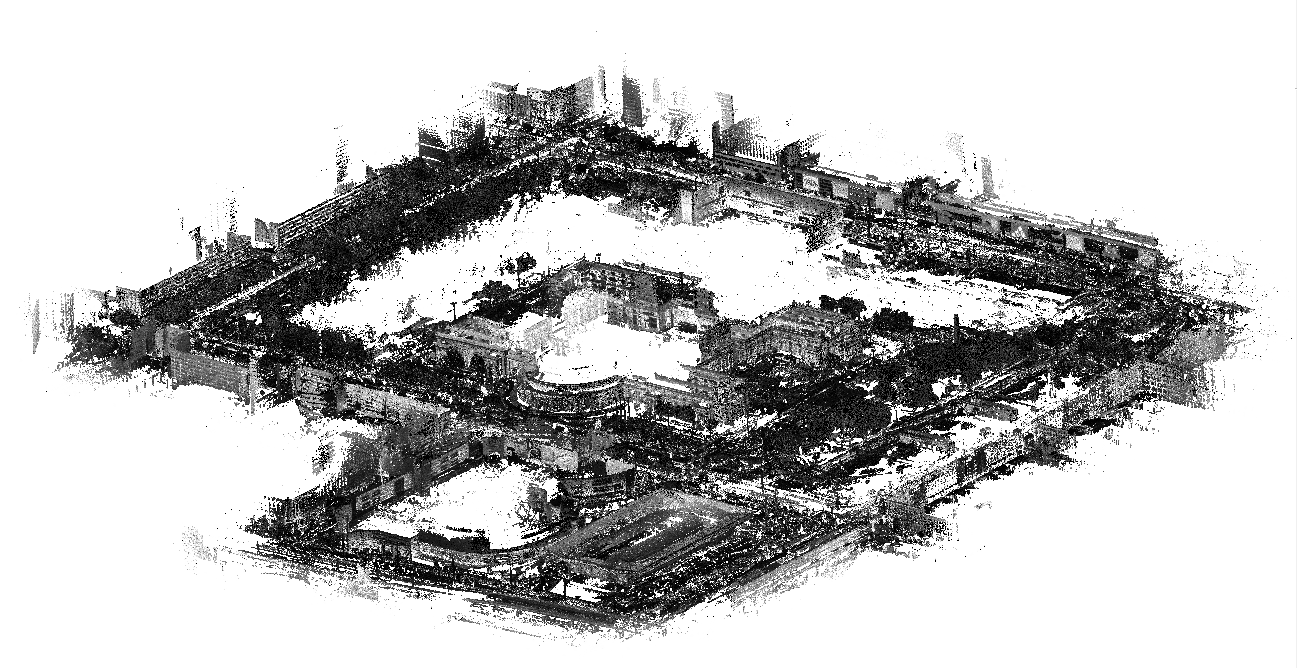
\includegraphics[width=1\linewidth]{cloud0}
	 	\caption{ContinousScanning\_0000}
	 \end{figure}
	\begin{figure}[H]
		\centering
		\begin{subfigure}{.90\textwidth}
			\centering
			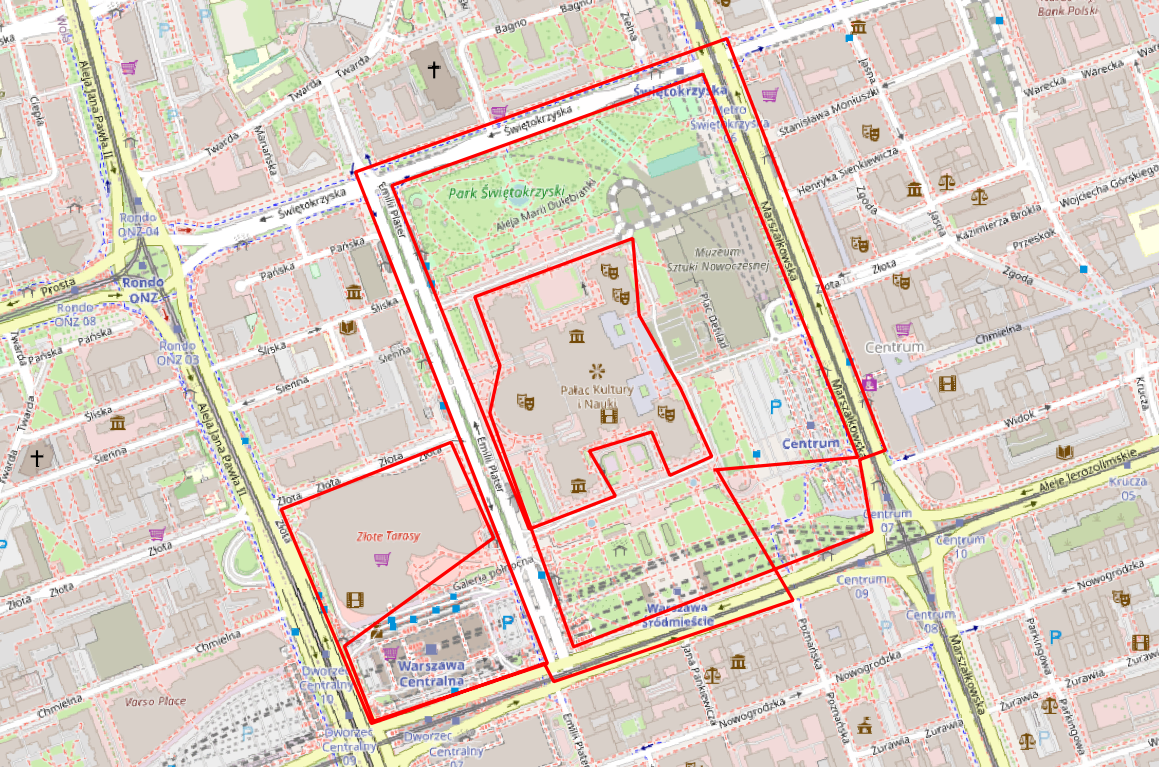
\includegraphics[width=1\linewidth]{route_p0}
			\caption{Planned route}
			\label{fig:a0}
		\end{subfigure}%
		\linebreak
		\begin{subfigure}{.90\textwidth}
			\centering
			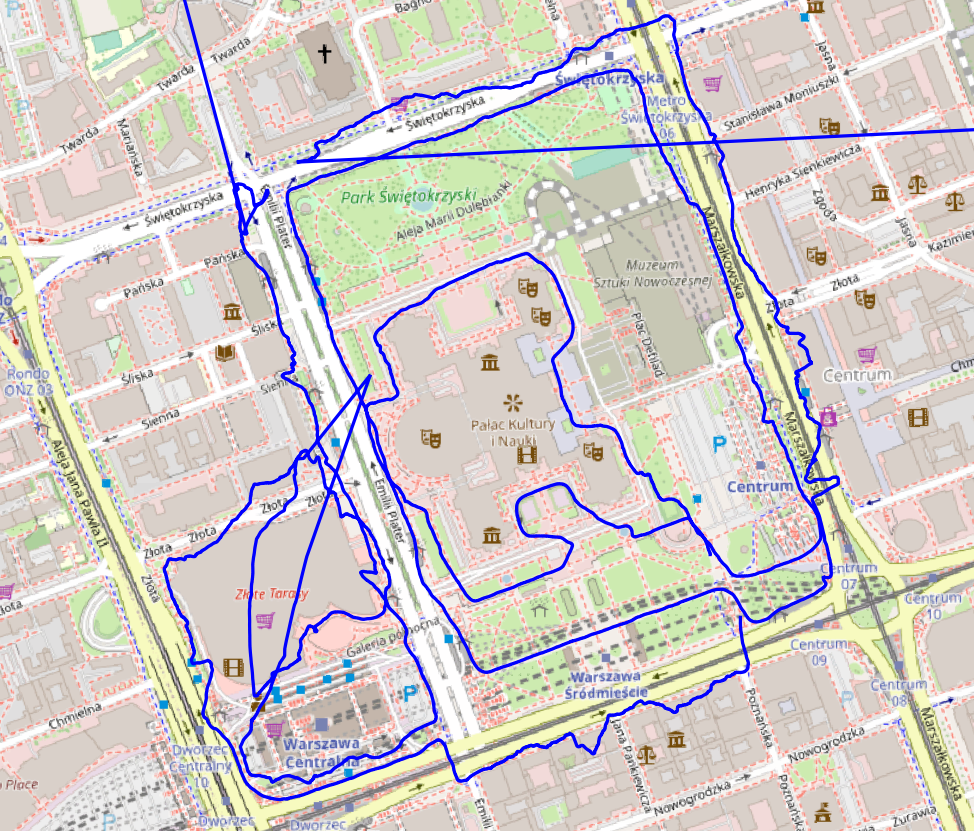
\includegraphics[width=1\linewidth]{route_c0}
			\caption{Covered route}
			\label{fig:b0}
		\end{subfigure}
		\caption{Scan 0000 planned and covered routes.}
		\label{fig:fig0}
	\end{figure}	
	\item \textbf{14.09.2023} Scan 0001. \\
	Second scan on Thursday was the one to test second 360 recording mode - Time Lapse. It performed significantly better than normal video as the battery went down to roughly \verb|40%| and localization proved to be more precise without such enormous errors. With prolonged battery working time I could achieve almost 10km distance (more precisely 9,64km (Fig. \ref{fig:b1})) of the planned 9,46 (Fig. \ref{fig:a1}). However such long routes proved to be too exhausting to be conducted five days a week for the next 2 months and thus daily track length was lowered to approximately 5km. After this scan, Friday was a day to rest, since I couldn't perform any more scans due to fatigue. 
	\begin{figure}[H]
		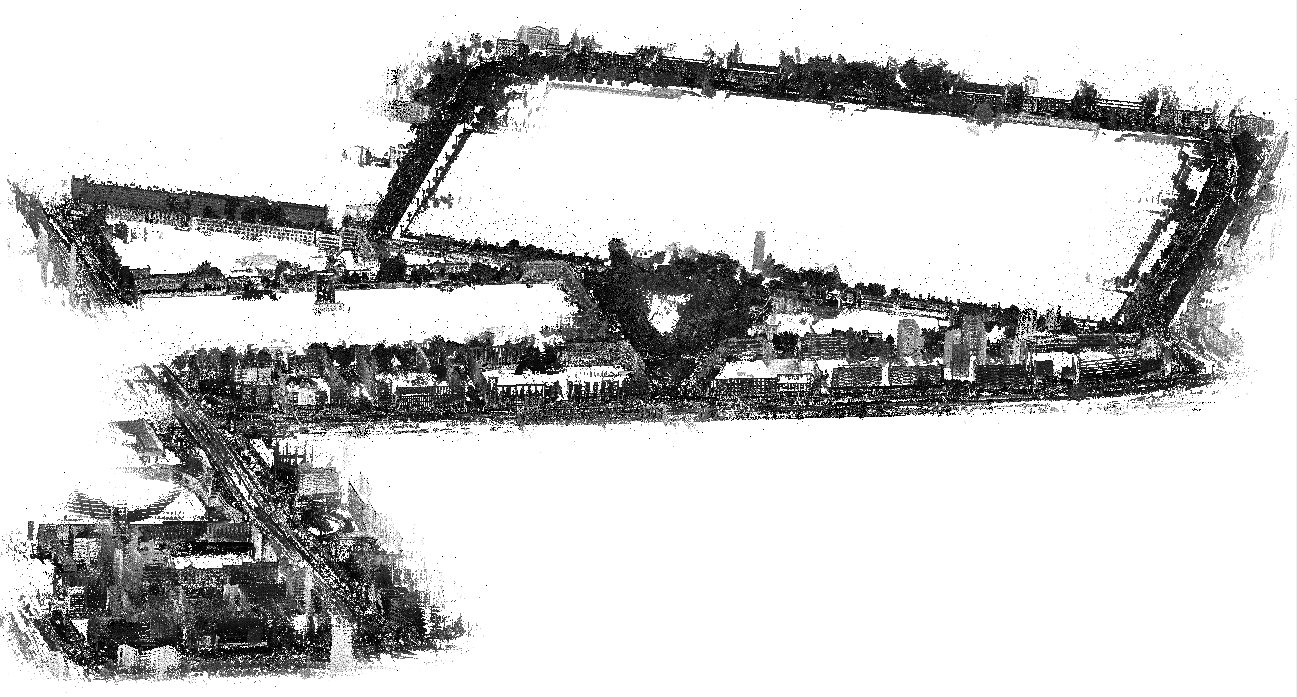
\includegraphics[width=1\linewidth]{cloud1}
		\caption{ContinousScanning\_0001}
	\end{figure}
	\begin{figure}[H]
		\centering
		\begin{subfigure}{.88\textwidth}
			\centering
			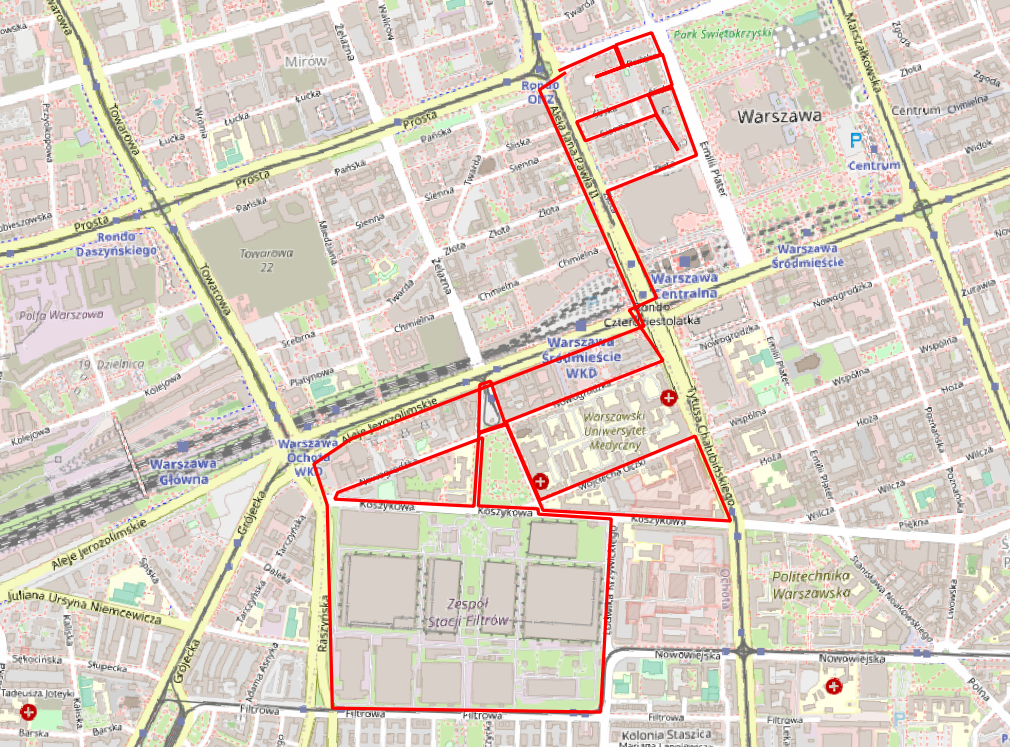
\includegraphics[width=1\linewidth]{route_p1}
			\caption{Planned route}
			\label{fig:a1}
		\end{subfigure}%
		\linebreak
		\begin{subfigure}{.88\textwidth}
			\centering
			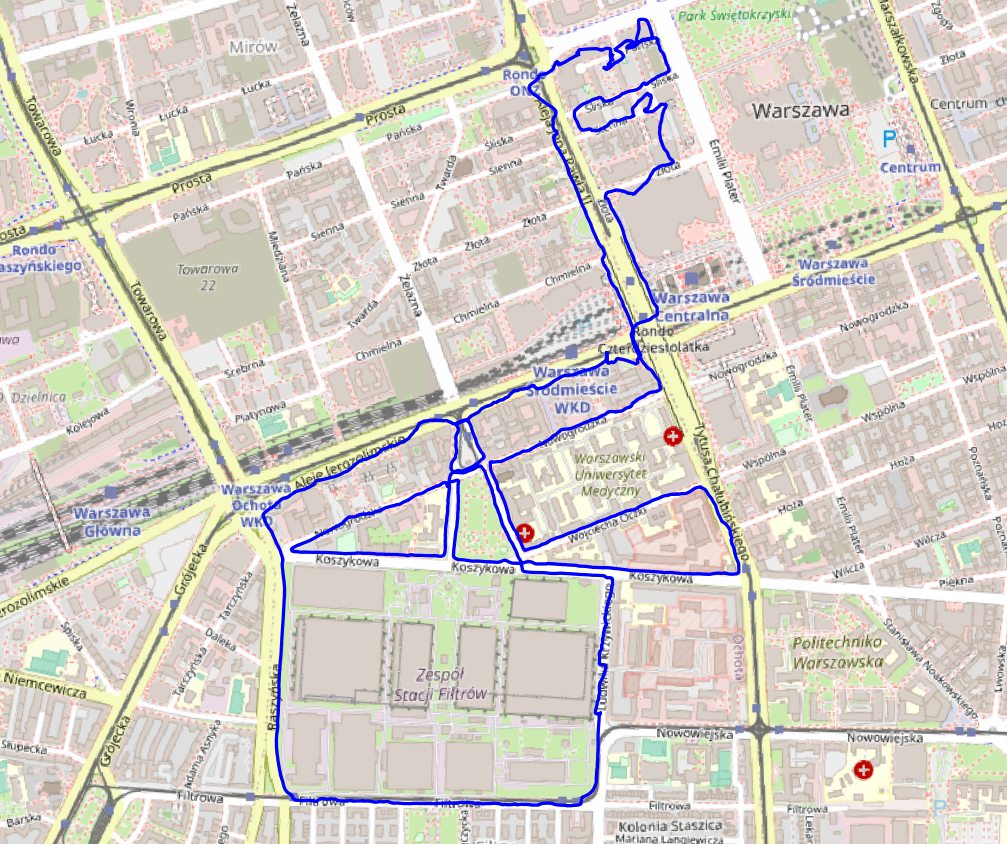
\includegraphics[width=1\linewidth]{route_c1}
			\caption{Covered route}
			\label{fig:b1}
		\end{subfigure}
		\caption{Scan 0001 planned and covered routes.}
		\label{fig:fig1}
	\end{figure}
\end{enumerate}
A vital conclusion after the first test scans is that Time Lapse mode should be utilized for scanning purposes due to its higher GPS accuracy and lower battery usage resulting in longer and more precise scans.
\section{Week 18-22 September 2023}
Scans conducted: continousScanning\_0002, continousScanning\_0003, continousScanning\_0004, continousScanning\_0005, continousScanning\_0006.\\

It was a first week with fully planned scans and a complete setup. 
\begin{enumerate}
	\item \textbf{18.09.2023} Scan 0002. \\
	On Monday, after the weekend rest, I conducted the first scan. It included all streets in an area beetwen Jerozolimskie avenue, Prosta street, Zelazna street and Jana Pawla II avenue. The planned route (Fig. \ref{fig:a2}) was estimated to be 6,48km but the covered route (Fig. \ref{fig:b2}) ended up to be a little bit higher - 6,59km which took 1 hour 21 minutes. The difference was caused by the need to scan a parking lot and an alley next to a skyscraper located between Chmielna street and Jerozolimskie avenue and probably because, as seen in the figure 3b, there appeared to be a localization problems in smartwach software.
	\begin{figure}[H]
		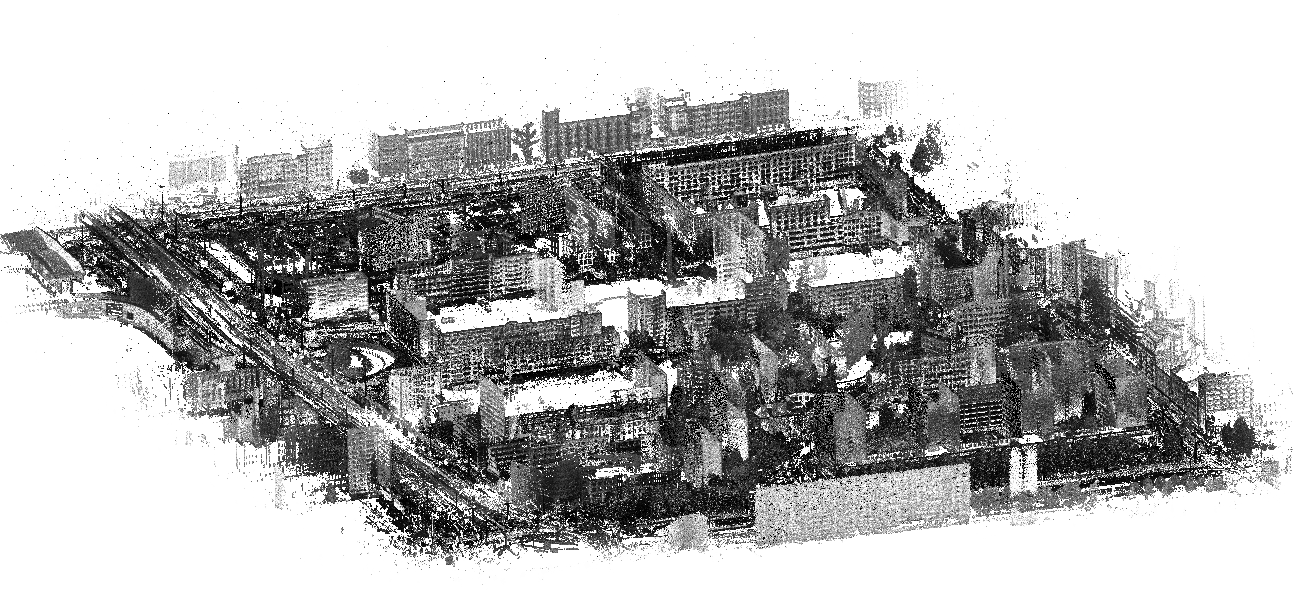
\includegraphics[width=1\linewidth]{cloud2}
		\caption{ContinousScanning\_0002}
	\end{figure}
	\begin{figure}[H]
		\centering
		\begin{subfigure}{.90\textwidth}
			\centering
			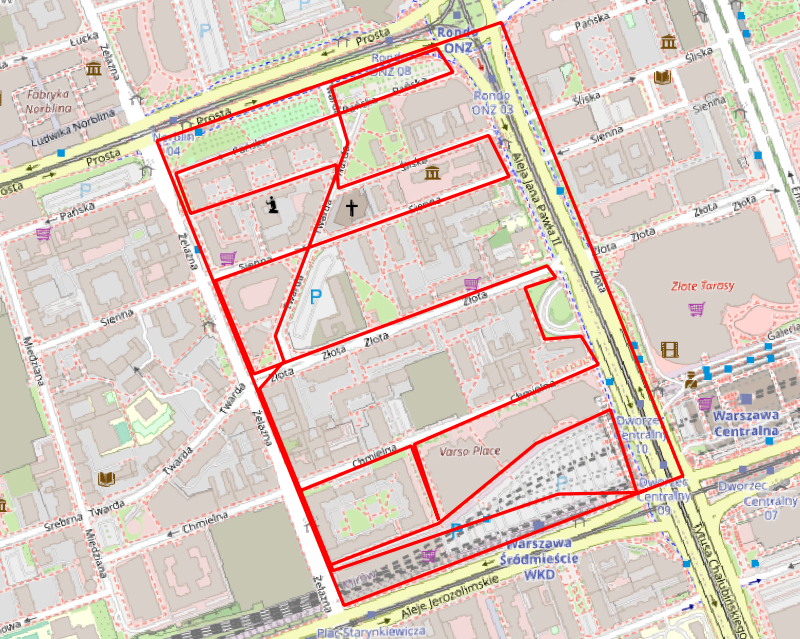
\includegraphics[width=1\linewidth]{route_p2}
			\caption{Planned route}
			\label{fig:a2}
		\end{subfigure}%
		\linebreak
		\begin{subfigure}{.90\textwidth}
			\centering
			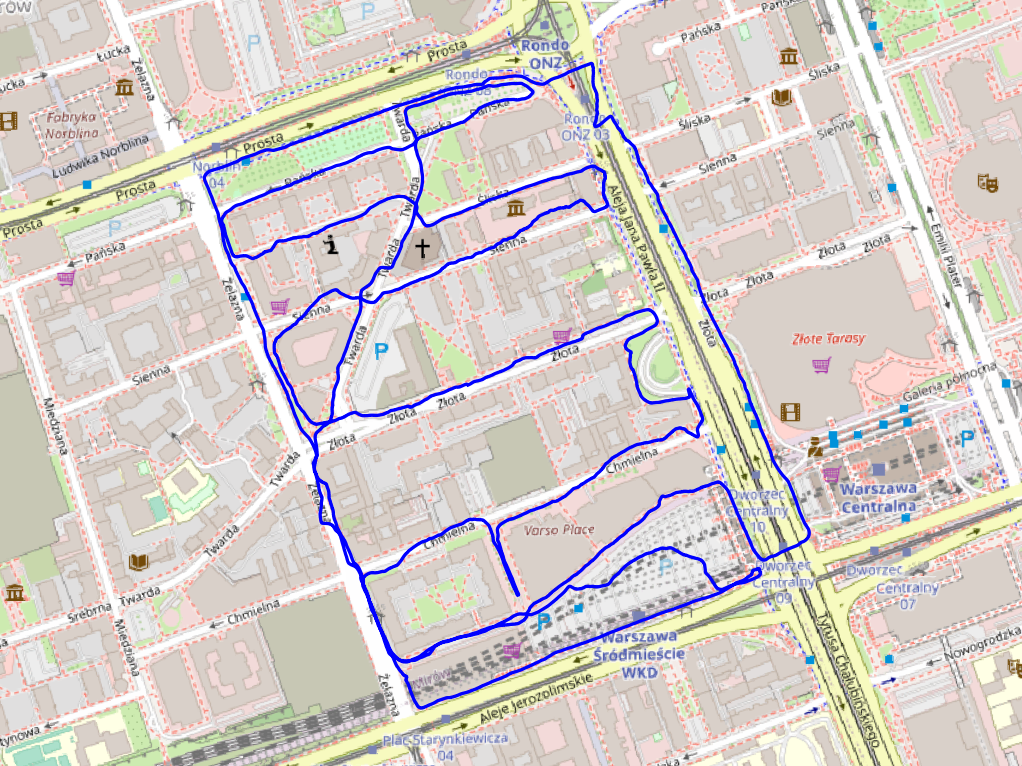
\includegraphics[width=1\linewidth]{route_c2}
			\caption{Covered route}
			\label{fig:b2}
		\end{subfigure}
		\caption{Scan 0002 planned and covered routes.}
		\label{fig:fig2}
	\end{figure}
	\item \textbf{19.09.2023} Scan 0003. \\
	Next day on Tuesday area between Jerozolimskie avenue, Wspolna street, Chalubinskiego street and Marszalkowska street was scanned. Planned route measured 4,82km (Fig. \ref{fig:a3}) and covered route 5,85km (Fig. \ref{fig:b3}). Difference was caused again probably by localization problems in smartwach but also by my additional routes near Srodmiescie district office and Saint Barbara church.
	\begin{figure}[H]
		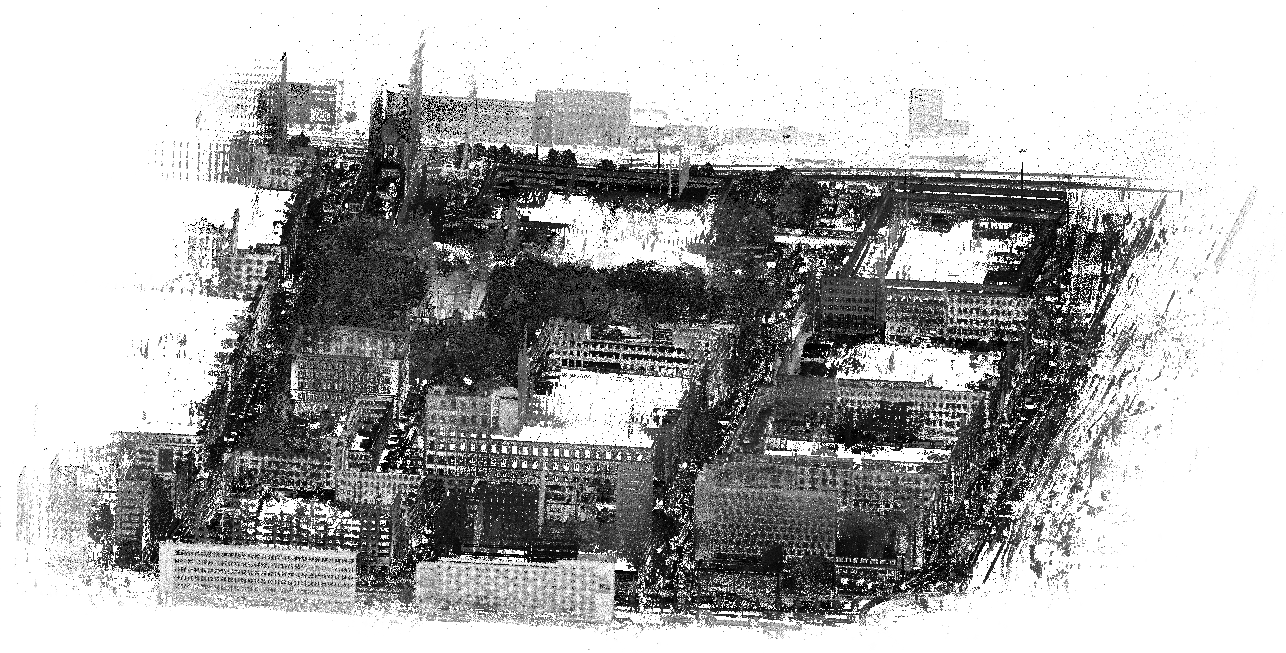
\includegraphics[width=1\linewidth]{cloud3}
		\caption{ContinousScanning\_0003}
	\end{figure}
	\begin{figure}[H]
		\centering
		\begin{subfigure}{.95\textwidth}
			\centering
			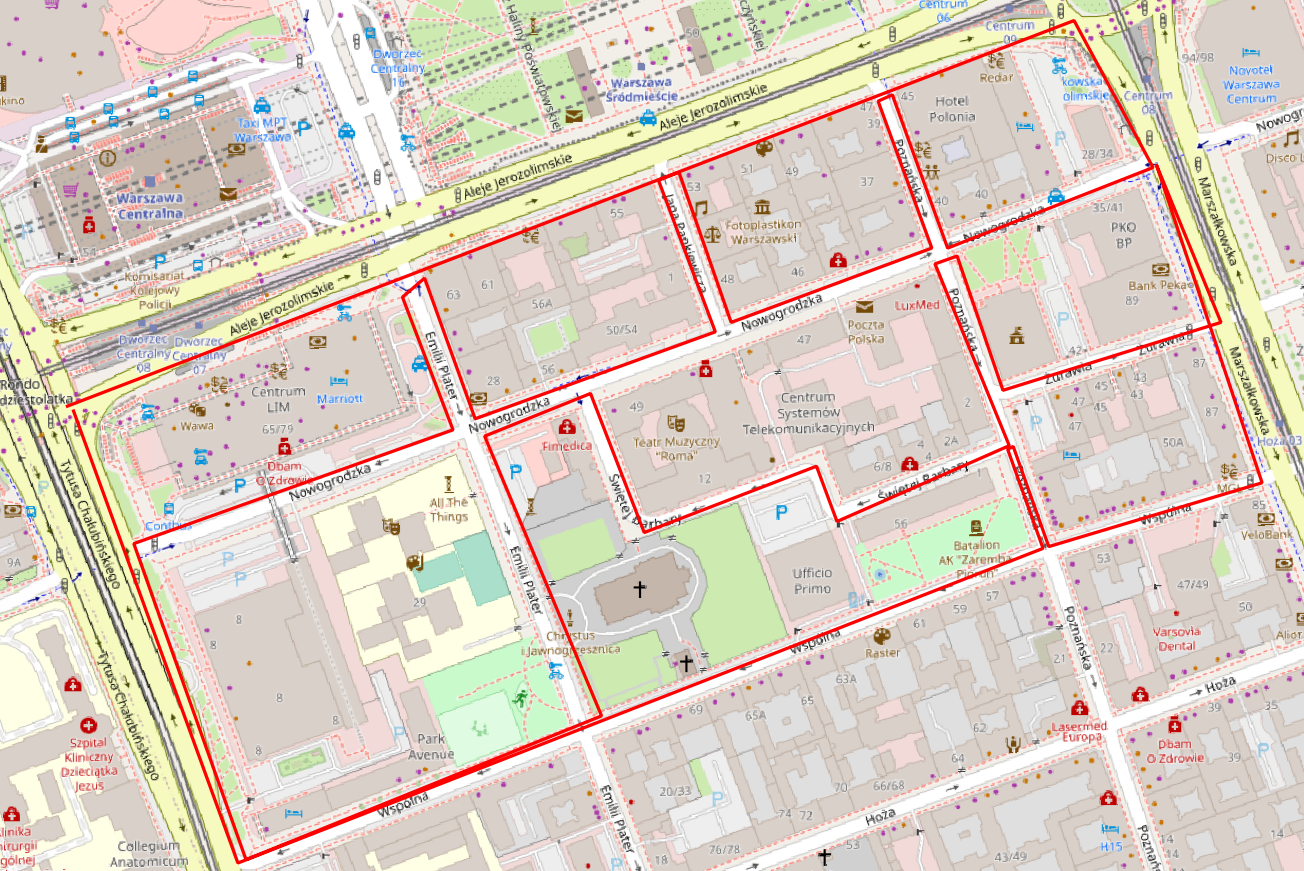
\includegraphics[width=1\linewidth]{route_p3}
			\caption{Planned route}
			\label{fig:a3}
		\end{subfigure}%
		\linebreak
		\begin{subfigure}{.95\textwidth}
			\centering
			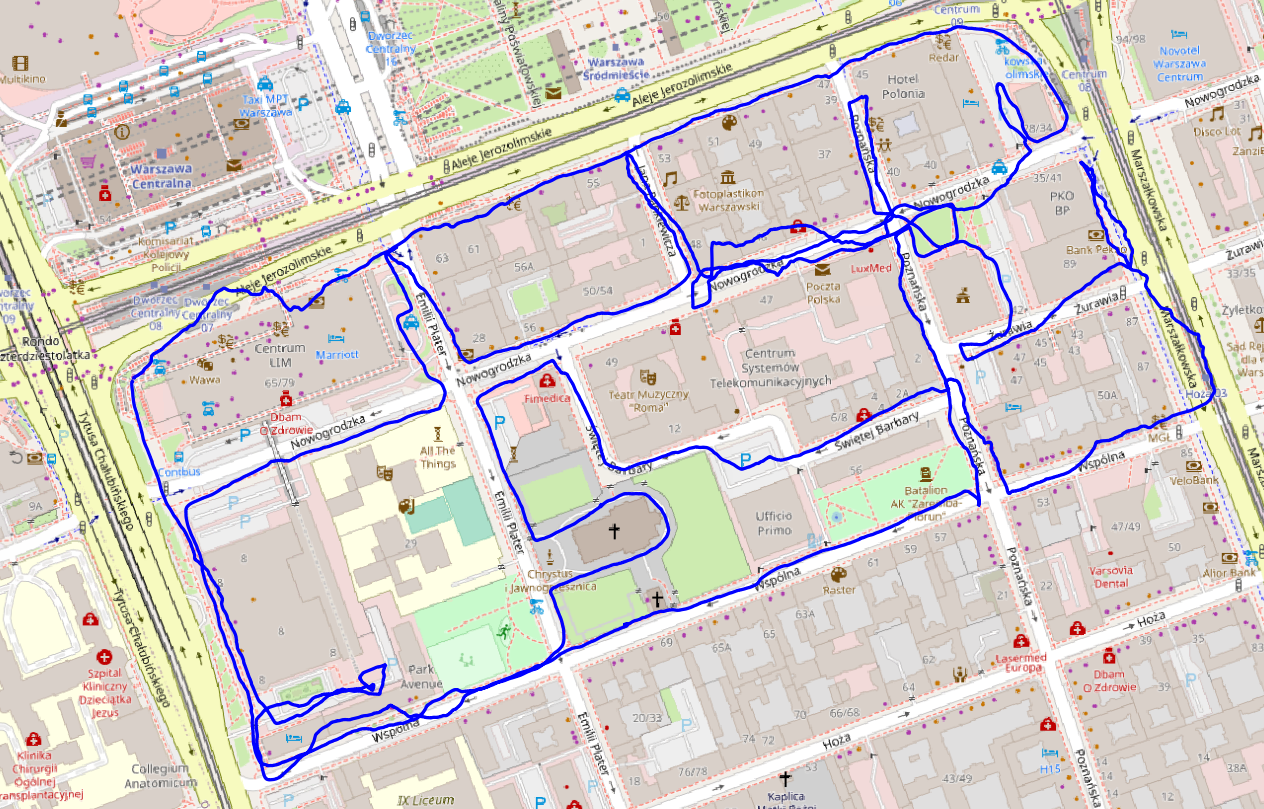
\includegraphics[width=1\linewidth]{route_c3}
			\caption{Covered route}
			\label{fig:b3}
		\end{subfigure}
		\caption{Scan 0003 planned and covered routes.}
		\label{fig:fig3}
	\end{figure}
	\pagebreak
	\item \textbf{20.09.2023} Scan 0004. \\
	On this day scanning was performed near the area from the day before, just a bit south, it included streets between Wspolna street, Koszykowa street, Chalubinskiego street and Marszalkowska street and also a fragment of Chalubinskiego street. Planned route was estimated to 5,06km (Fig. \ref{fig:a4}) and ultimately reached similar distance: 4,99km (Fig. \ref{fig:b4}).
	\begin{figure}[H]
		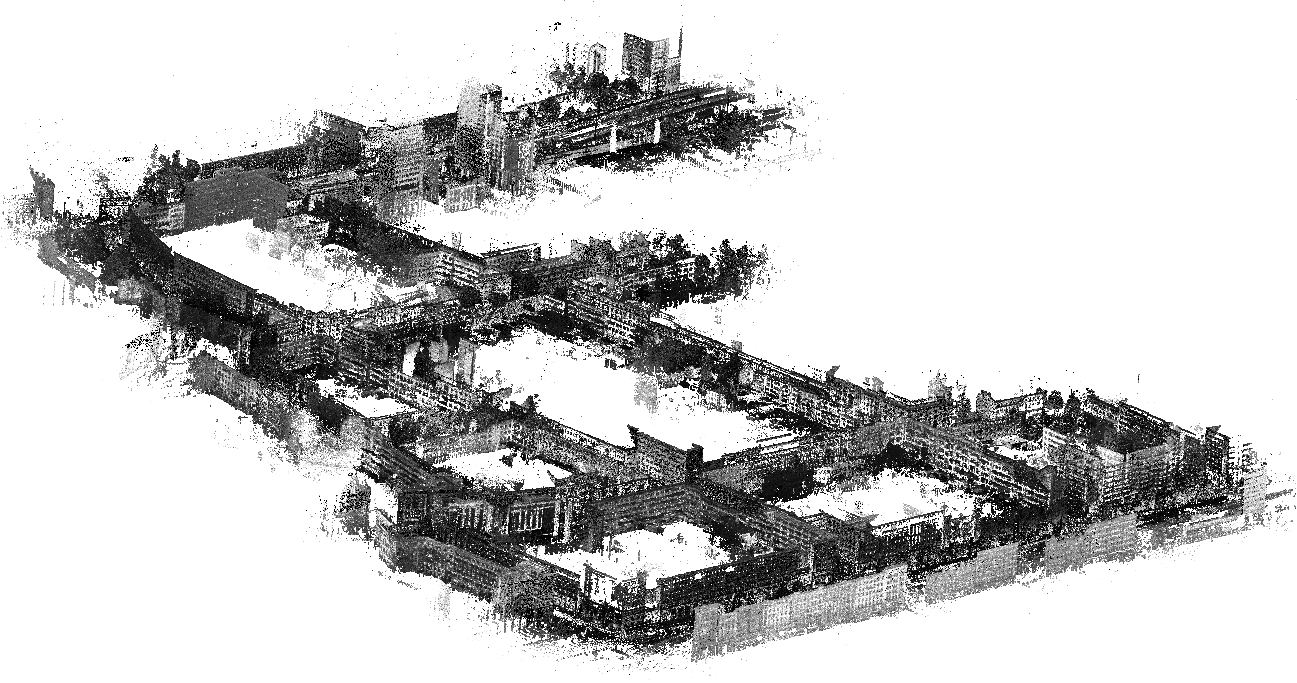
\includegraphics[width=1\linewidth]{cloud4}
		\caption{ContinousScanning\_0004}
	\end{figure}
	\begin{figure}[H]
	\centering
	\begin{subfigure}{1\textwidth}
		\centering
		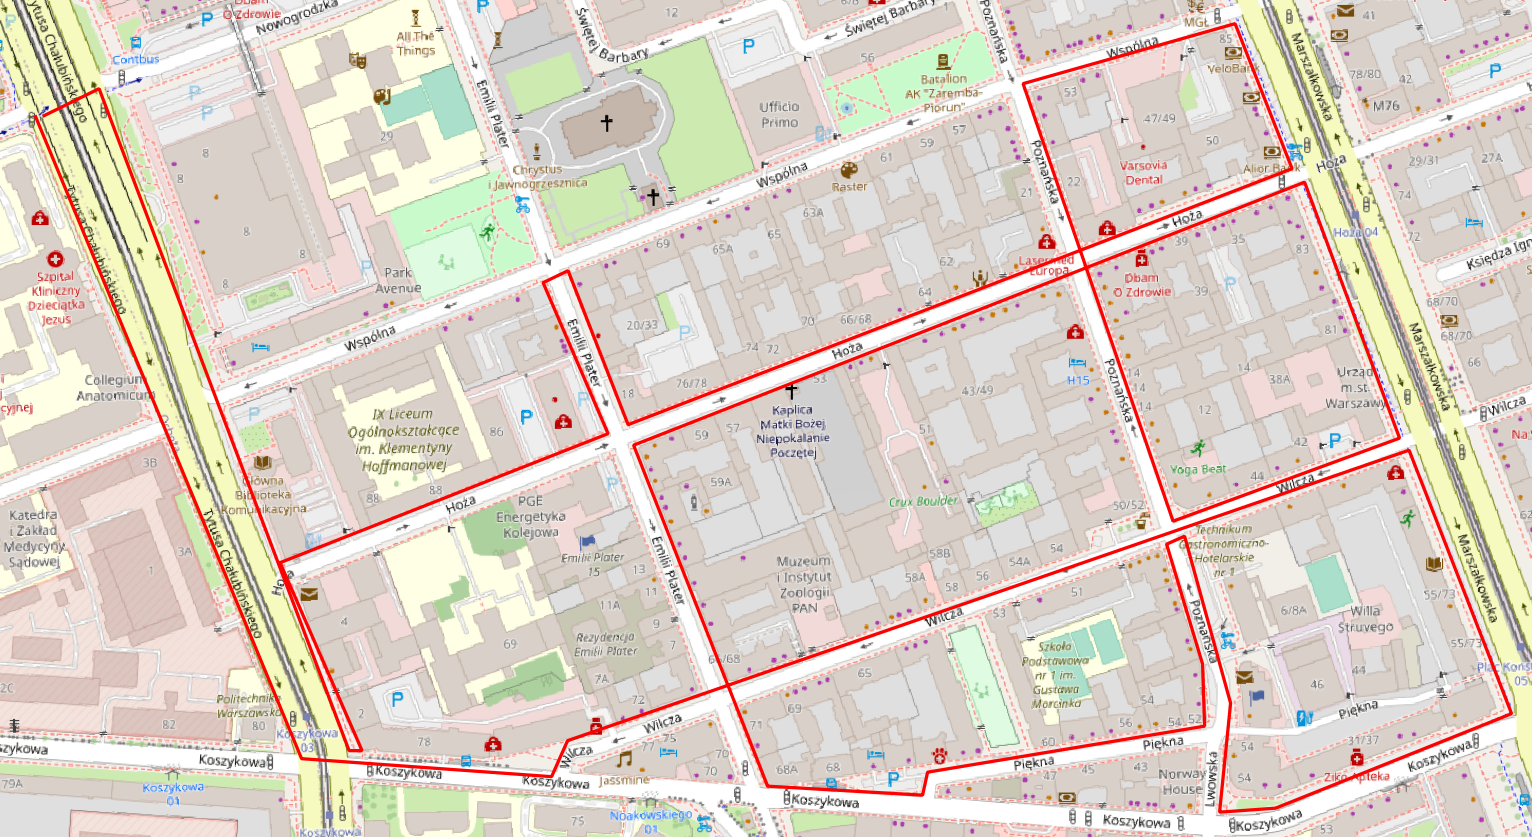
\includegraphics[width=1\linewidth]{route_p4}
		\caption{Planned route}
		\label{fig:a4}
	\end{subfigure}%
	\linebreak
	\begin{subfigure}{1\textwidth}
		\centering
		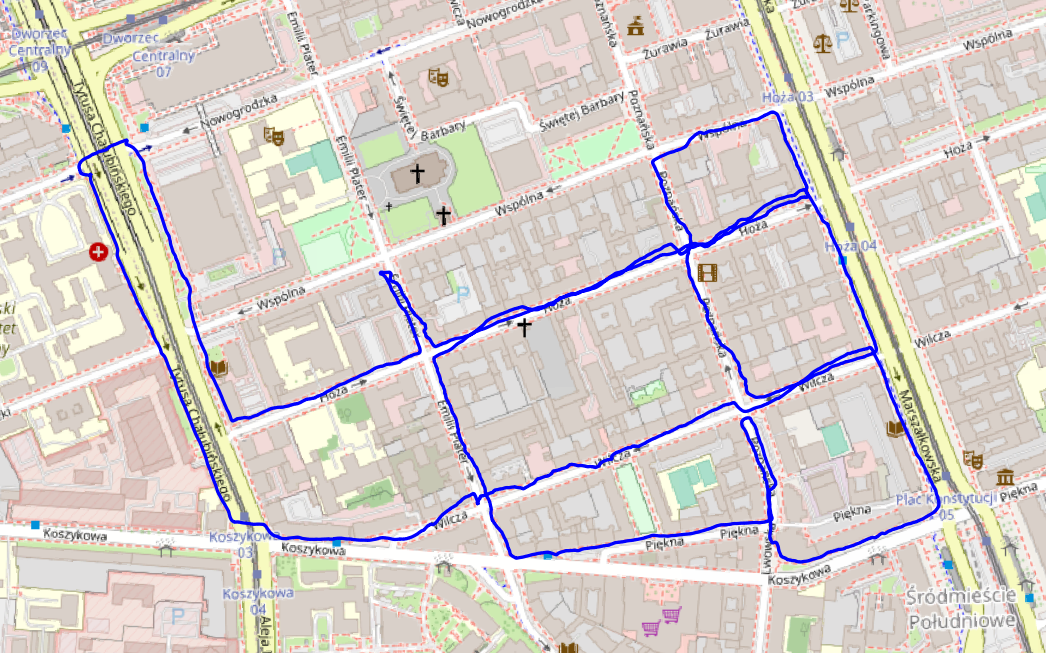
\includegraphics[width=1\linewidth]{route_c4}
		\caption{Covered route}
		\label{fig:b4}
	\end{subfigure}
	\caption{Scan 0004 planned and covered routes.}
	\label{fig:fig4}
\end{figure}
\pagebreak
\item \textbf{21.09.2023} Scan 0005. \\
That day scanning area encompassed Marszalkowska street, Constitution Square and surroundings around the main campus of Warsaw University of Technology. Planned route (Fig. \ref{fig:a5}) was 5,78km and covered route (Fig. \ref{fig:b5}), as well as most of the previous ones, exceeded this distance and summed up to  6,44km. 
\begin{figure}[H]
	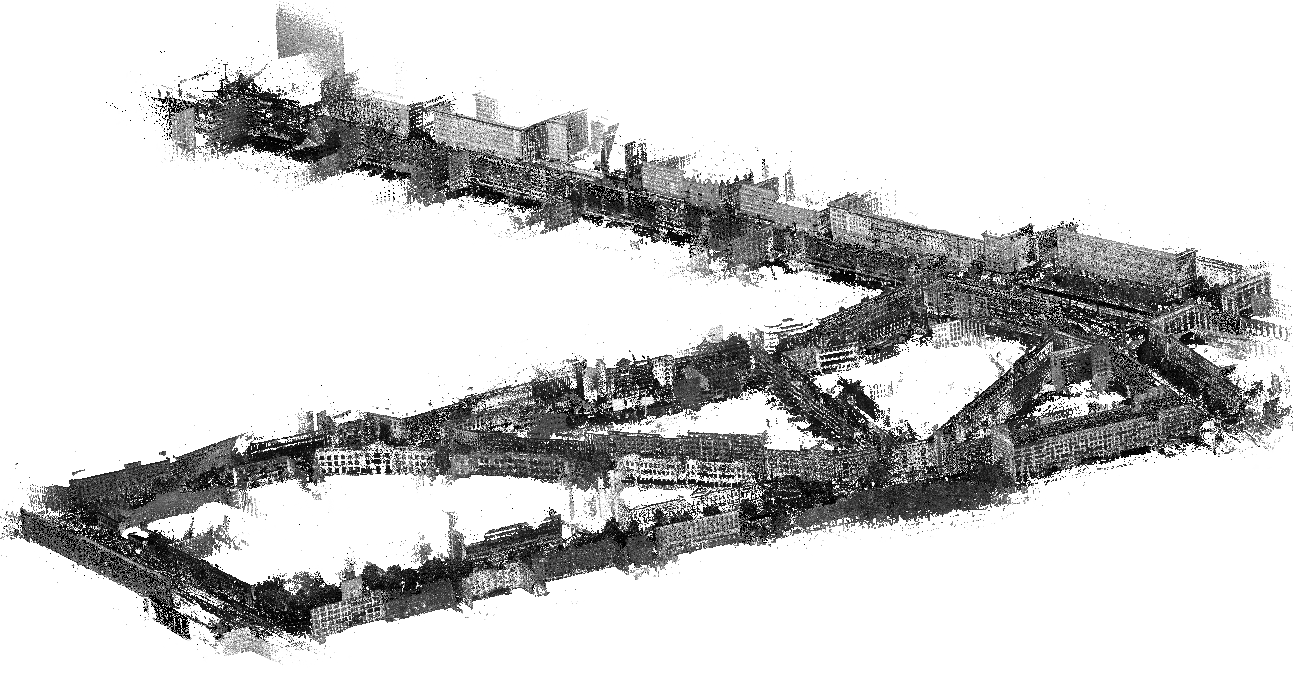
\includegraphics[width=1\linewidth]{cloud5}
	\caption{ContinousScanning\_0005}
\end{figure}
\begin{figure}[H]
	\centering
	\begin{subfigure}{.80\textwidth}
		\centering
		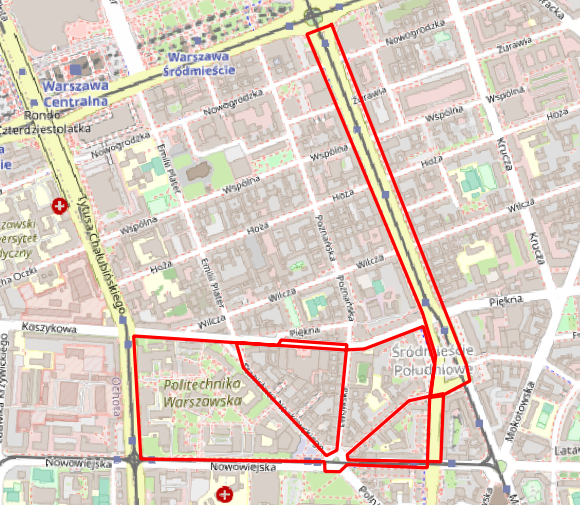
\includegraphics[width=1\linewidth]{route_p5}
		\caption{Planned route}
		\label{fig:a5}
	\end{subfigure}%
	\linebreak
	\begin{subfigure}{.80\textwidth}
		\centering
		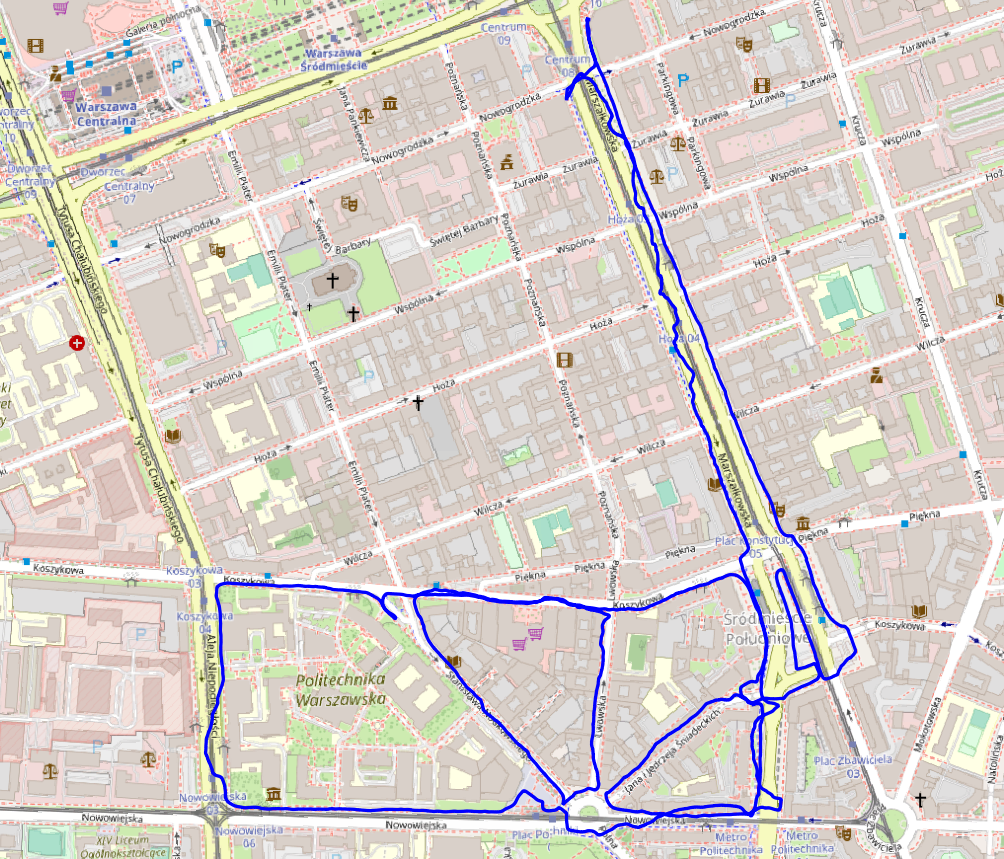
\includegraphics[width=1\linewidth]{route_c5}
		\caption{Covered route}
		\label{fig:b5}
	\end{subfigure}
	\caption{Scan 0005 planned and covered routes.}
	\label{fig:fig5}
\end{figure}
\item \textbf{22.09.2023} Scan 0006. \\
Scan was performed east of Marszalkowska street. Mostly it included Nowogrodzka street , Zurawia street, Wspolna street, Hoza street, Wilcza street and Krucza street. Planned route (Fig. \ref{fig:a6}) was estimated to 5,65km, but as happened before, covered route (Fig. \ref{fig:b6}) took longer and achieved 6,11km.
\begin{figure}[H]
	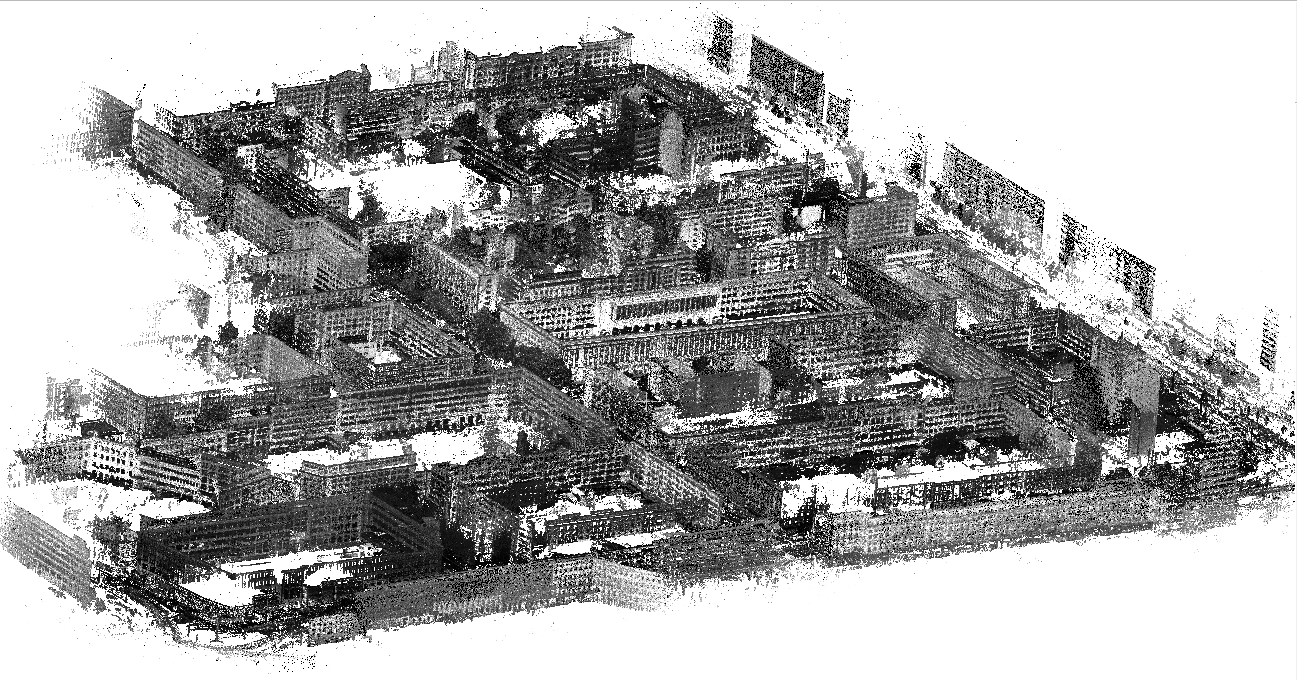
\includegraphics[width=1\linewidth]{cloud6}
	\caption{ContinousScanning\_0006}
\end{figure}
\begin{figure}[H]
	\centering
	\begin{subfigure}{.80\textwidth}
		\centering
		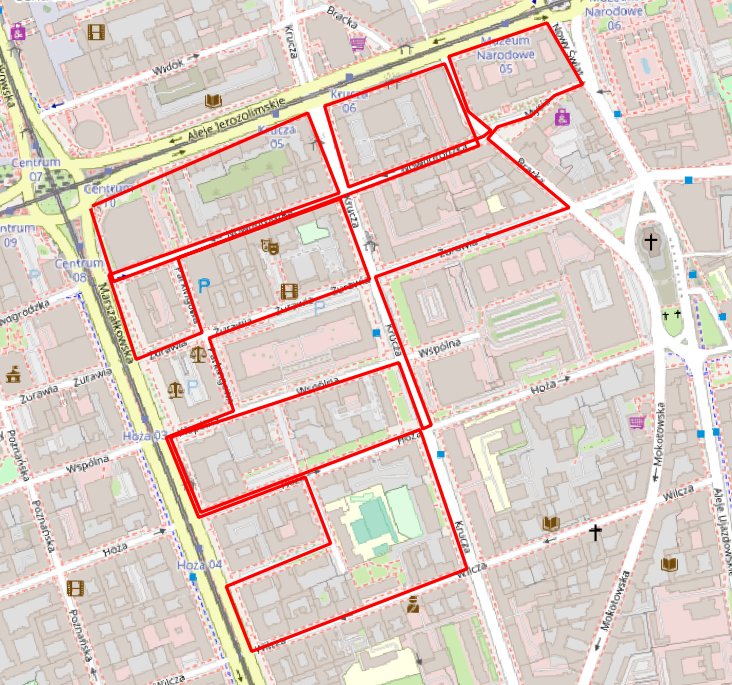
\includegraphics[width=1\linewidth]{route_p6}
		\caption{Planned route}
		\label{fig:a6}
	\end{subfigure}%
	\linebreak
	\begin{subfigure}{.80\textwidth}
		\centering
		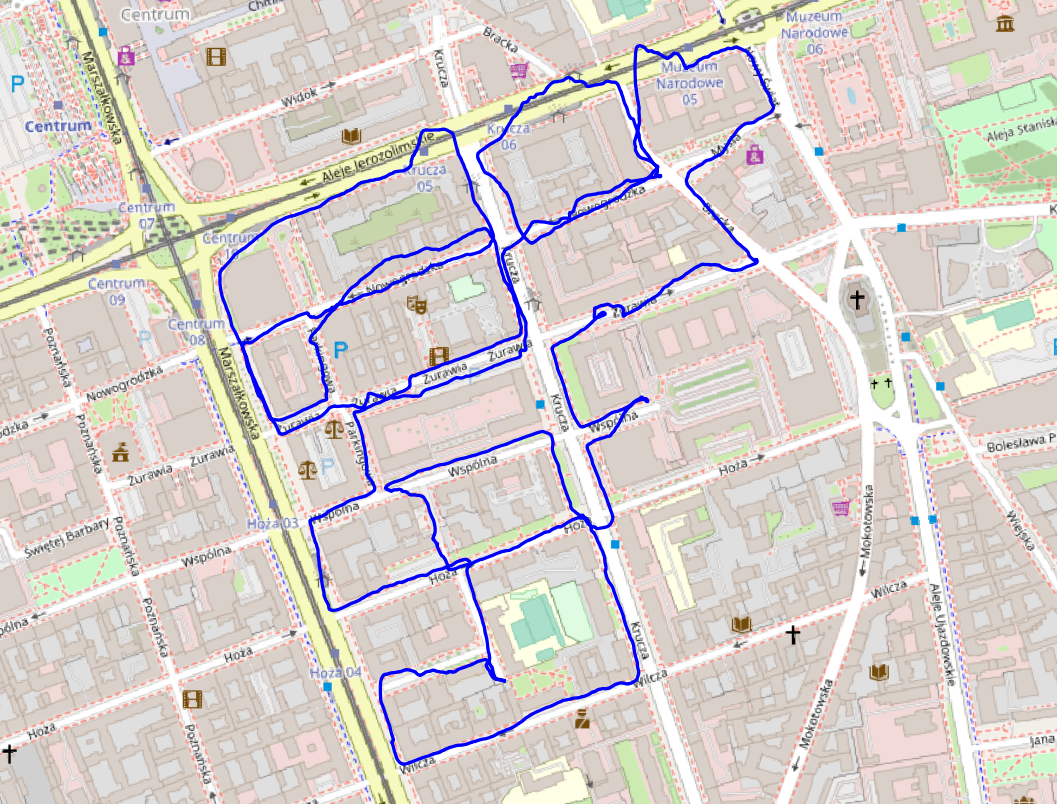
\includegraphics[width=1\linewidth]{route_c6}
		\caption{Covered route}
		\label{fig:b6}
	\end{subfigure}
	\caption{Scan 0006 planned and covered routes.}
	\label{fig:fig6}
\end{figure} 
\end{enumerate}

\section{Week 25-29 September 2023} 
Scans conducted: continousScanning\_0007, continousScanning\_0008, continousScanning\_0009, continousScanning\_0010, continousScanning\_0011.\\
\begin{enumerate}
	\item \textbf{25.09.2023} Scan 0007. \\
	Scan was planned to be conducted in neighbourhood of Three Crosses Square. Total route was calculated to be 5,77km (Fig. \ref{fig:a7}) but covered one (Fig. \ref{fig:b7}) amounted to 7,38km due to my endeavors to fully cover Wiejska street and precisely scan the square.
	\begin{figure}[H]
		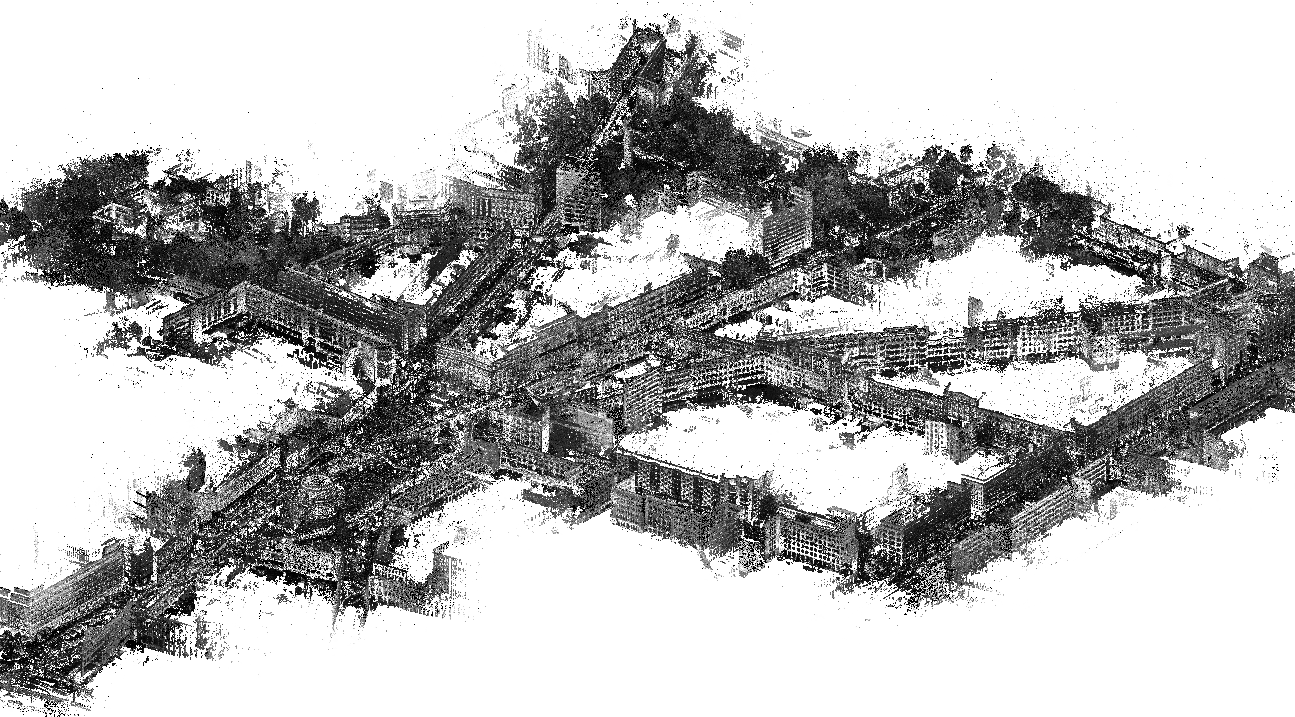
\includegraphics[width=1\linewidth]{cloud7}
		\caption{ContinousScanning\_0007}
	\end{figure}
	\begin{figure}[H]
		\centering
		\begin{subfigure}{.75\textwidth}
			\centering
			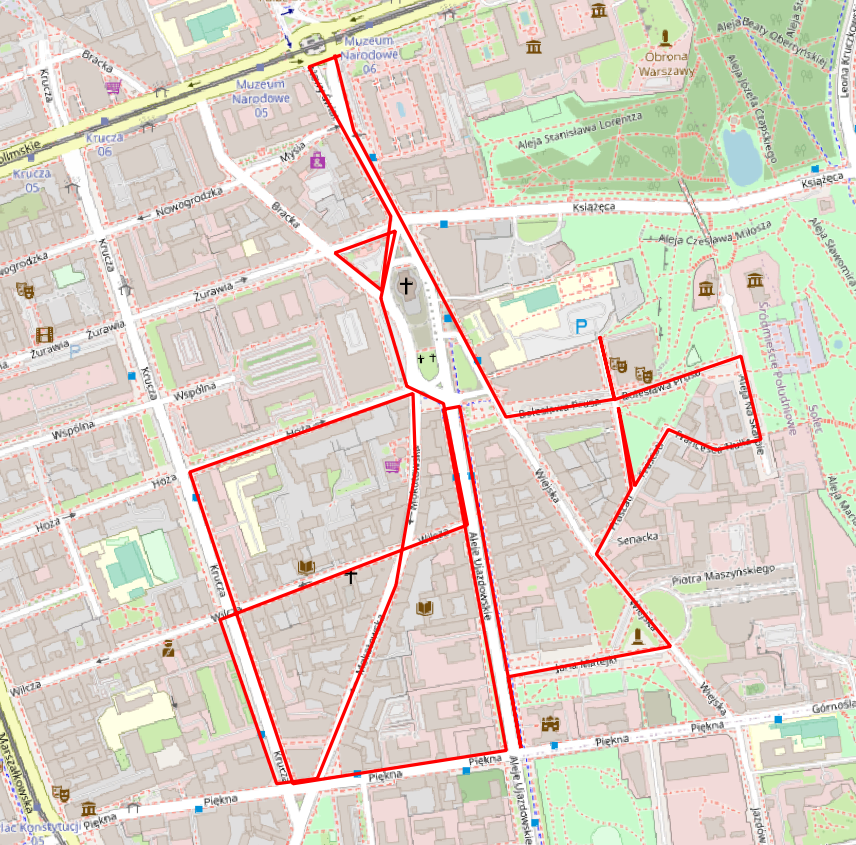
\includegraphics[width=1\linewidth]{route_p7}
			\caption{Planned route}
			\label{fig:a7}
		\end{subfigure}%
		\linebreak
		\begin{subfigure}{.75\textwidth}
			\centering
			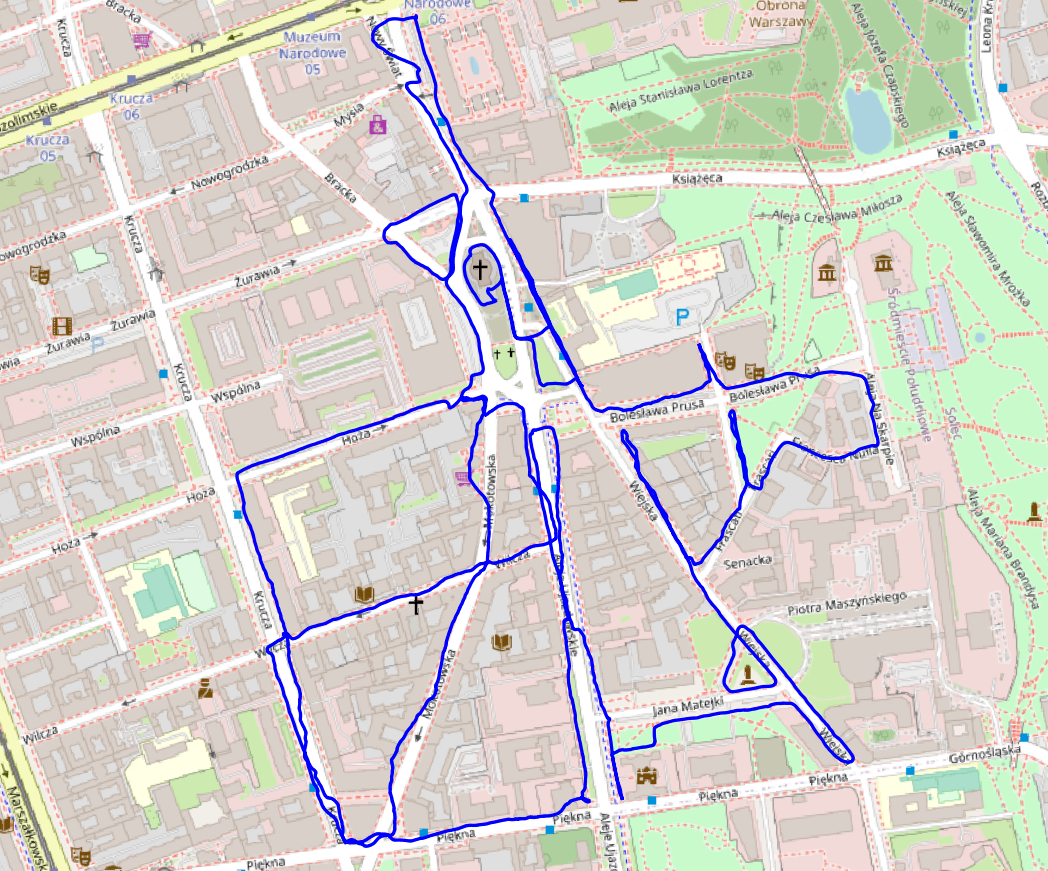
\includegraphics[width=1\linewidth]{route_c7}
			\caption{Covered route}
			\label{fig:b7}
		\end{subfigure}
		\caption{Scan 0007 planned and covered routes.}
		\label{fig:fig7}
	\end{figure} 
	\item \textbf{26.09.2023} Scan 0008. \\
	Planned route (Fig. \ref{fig:a8}) was estimated to 6,61km but covered route (Fig. \ref{fig:b8}) reached 6,89km, mostly because of my efforts to scan Warsaw Insurgents Square as thoroughly as possible. It wasn't as easy as I had expected since during the time I was performing scans the square was undergoing reconstruction.
	\begin{figure}[H]
		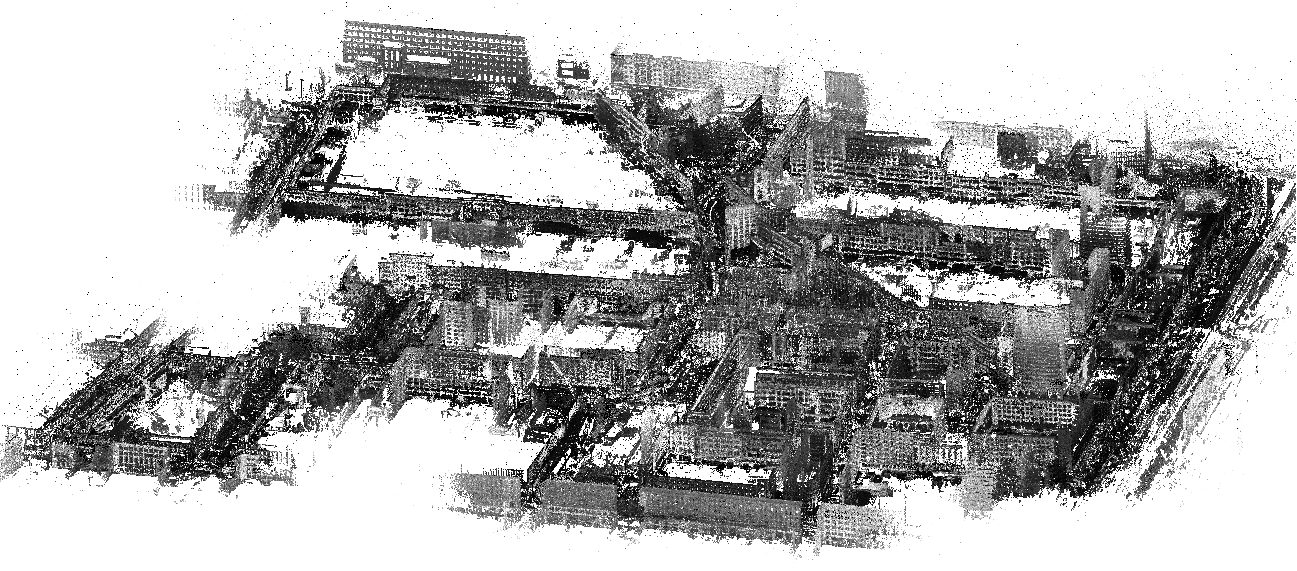
\includegraphics[width=1\linewidth]{cloud8}
		\caption{ContinousScanning\_0008}
	\end{figure}
	\begin{figure}[H]
		\centering
		\begin{subfigure}{.83\textwidth}
			\centering
			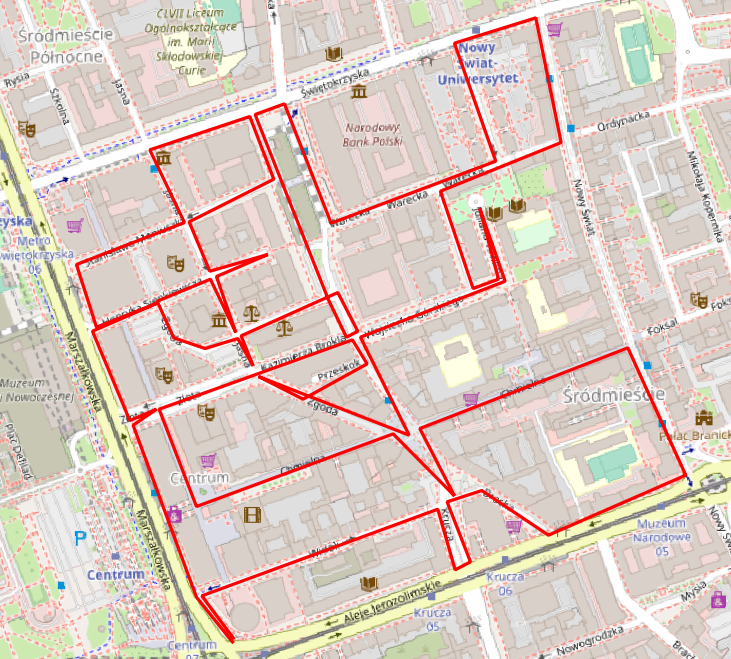
\includegraphics[width=1\linewidth]{route_p8}
			\caption{Planned route}
			\label{fig:a8}
		\end{subfigure}%
		\linebreak
		\begin{subfigure}{.83\textwidth}
			\centering
			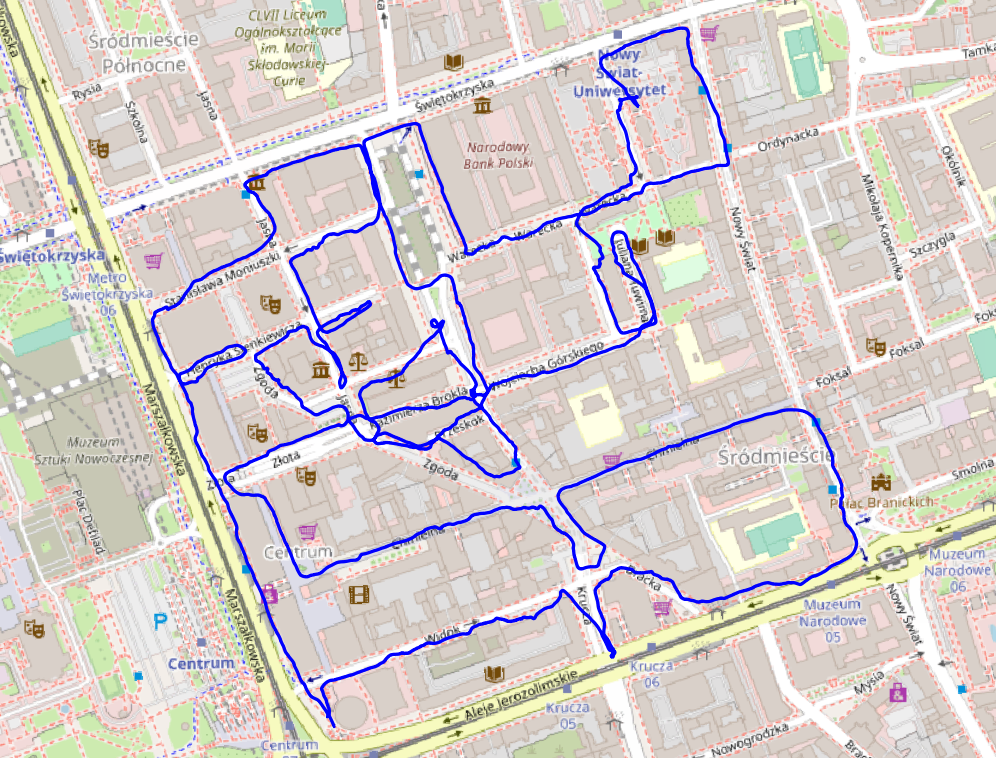
\includegraphics[width=1\linewidth]{route_c8}
			\caption{Covered route}
			\label{fig:b8}
		\end{subfigure}
		\caption{Scan 0008 planned and covered routes.}
		\label{fig:fig8}
	\end{figure} 
	\item \textbf{27.09.2023} Scan 0009. \\
	Region to be scanned included streets between Swietokrzyska street, Krolewska street, Jana Pawla II avenue and Nowy Swiat street and route was planned to be 5,34km long (Fig. \ref{fig:a9}). Longer covered route reached 5,82km (Fig. \ref{fig:b9}) because of my mistake during scanning, I skipped one street and had to come back + forgot to turn smart watch on and started recording after a few minutes.
	\begin{figure}[H]
		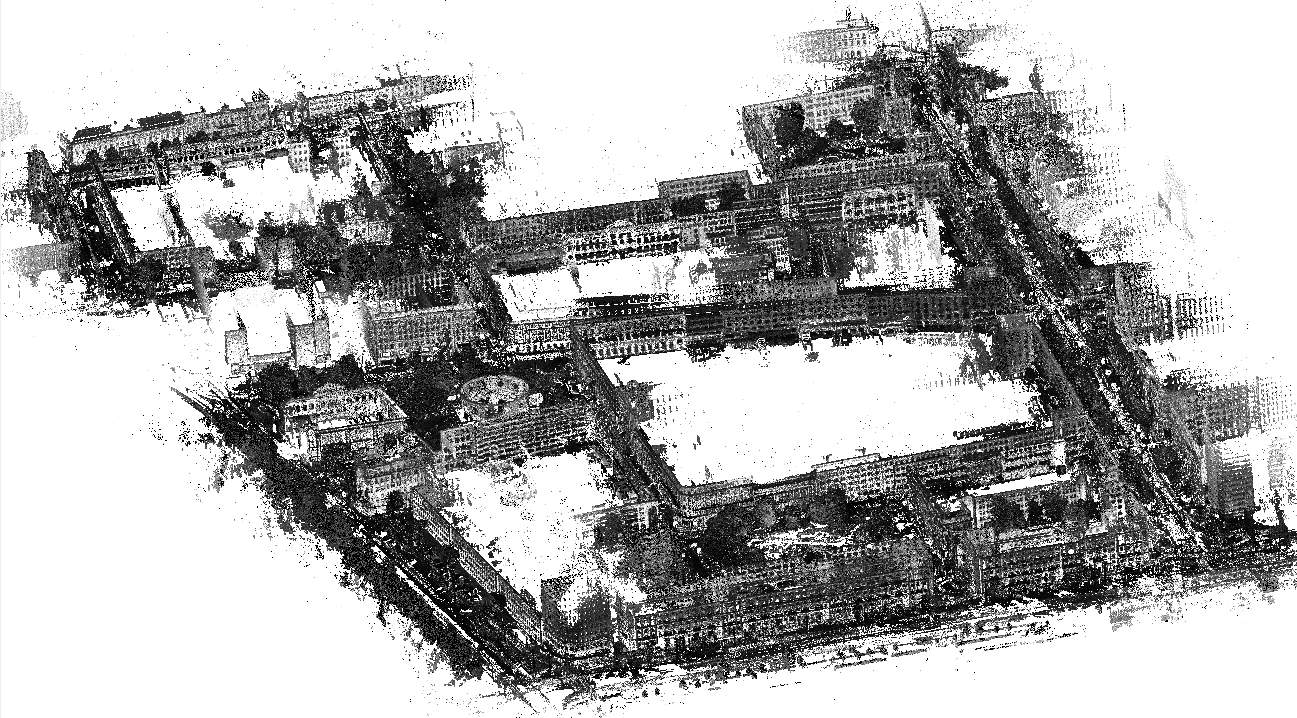
\includegraphics[width=1\linewidth]{cloud9}
		\caption{ContinousScanning\_0009}
	\end{figure}
	\begin{figure}[H]
		\centering
		\begin{subfigure}{.93\textwidth}
			\centering
			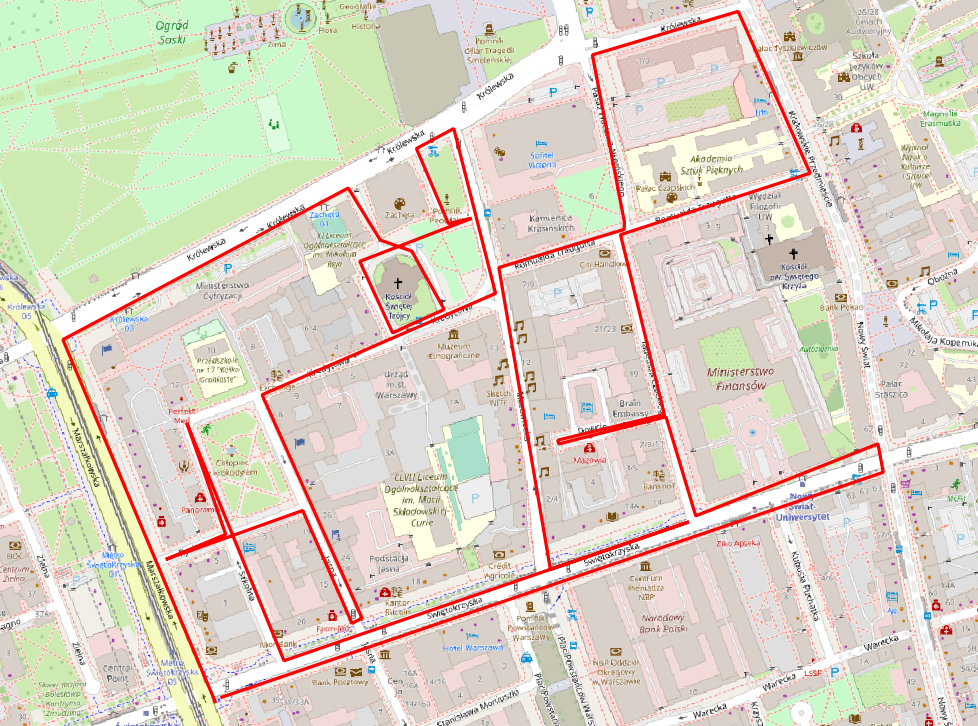
\includegraphics[width=1\linewidth]{route_p9}
			\caption{Planned route}
			\label{fig:a9}
		\end{subfigure}%
		\linebreak
		\begin{subfigure}{.93\textwidth}
			\centering
			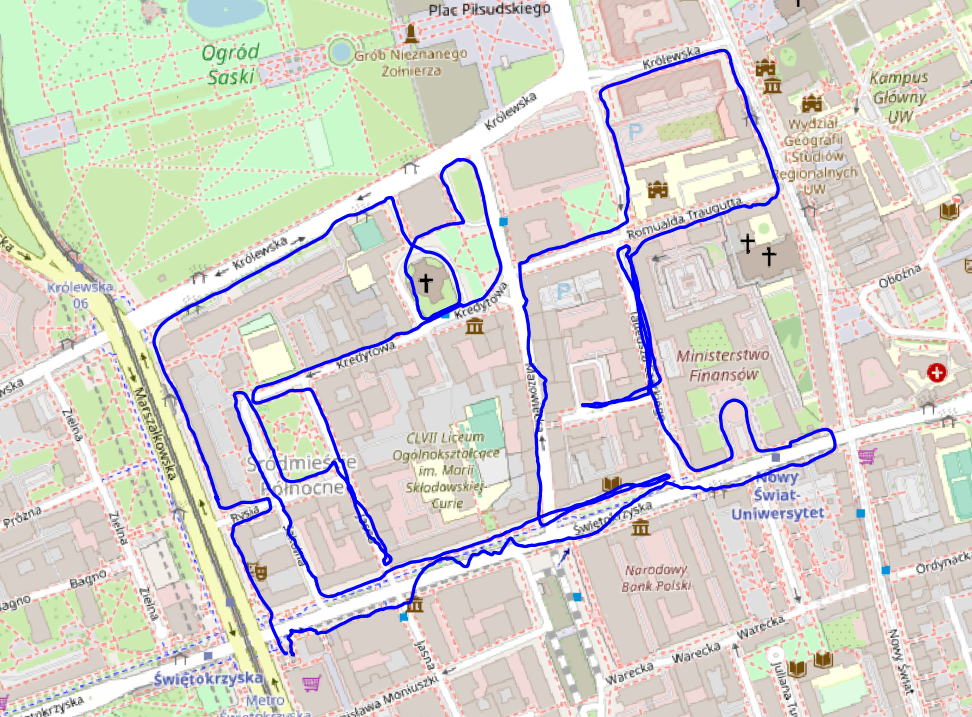
\includegraphics[width=1\linewidth]{route_c9}
			\caption{Covered route}
			\label{fig:b9}
		\end{subfigure}
		\caption{Scan 0009 planned and covered routes.}
		\label{fig:fig9}
	\end{figure} 
	\item \textbf{28.09.2023} Scan 0010. \\
	Planned route was approximated to 6,46km (Fig. \ref{fig:a10}), in neighbourhood of Mirowski square and streets north of Swietokrzyska street. Covered route 6,91km (Fig. \ref{fig:b10})
	\begin{figure}[H]
		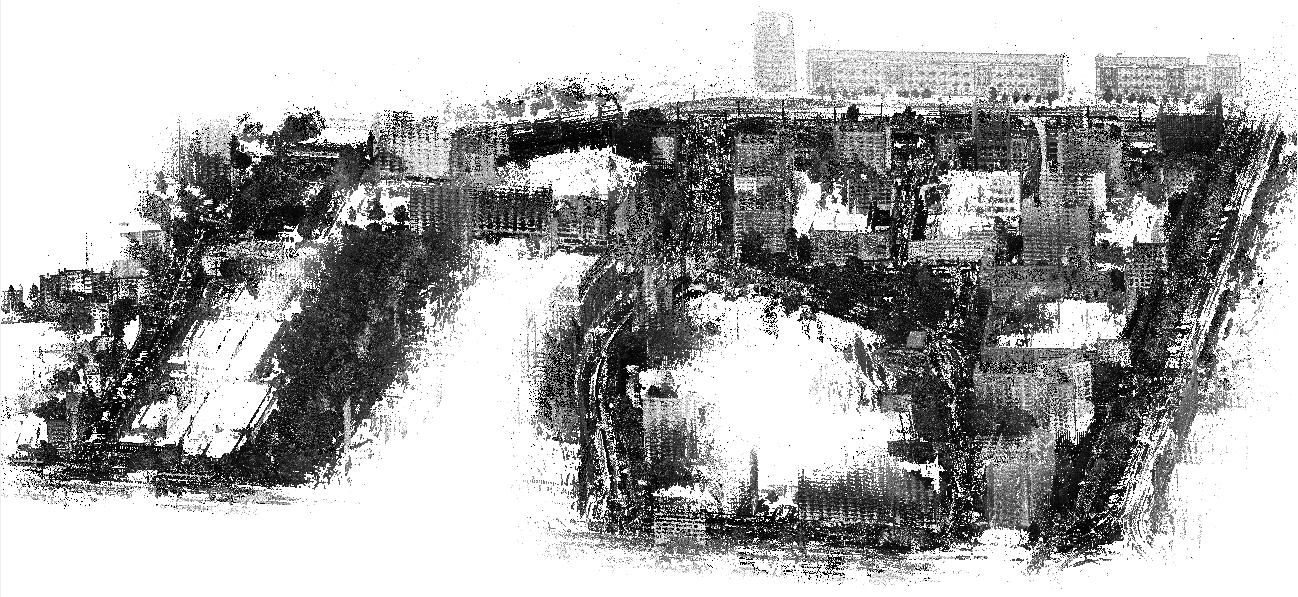
\includegraphics[width=1\linewidth]{cloud10}
		\caption{ContinousScanning\_0010}
	\end{figure}
	\begin{figure}[H]
		\centering
		\begin{subfigure}{.90\textwidth}
			\centering
			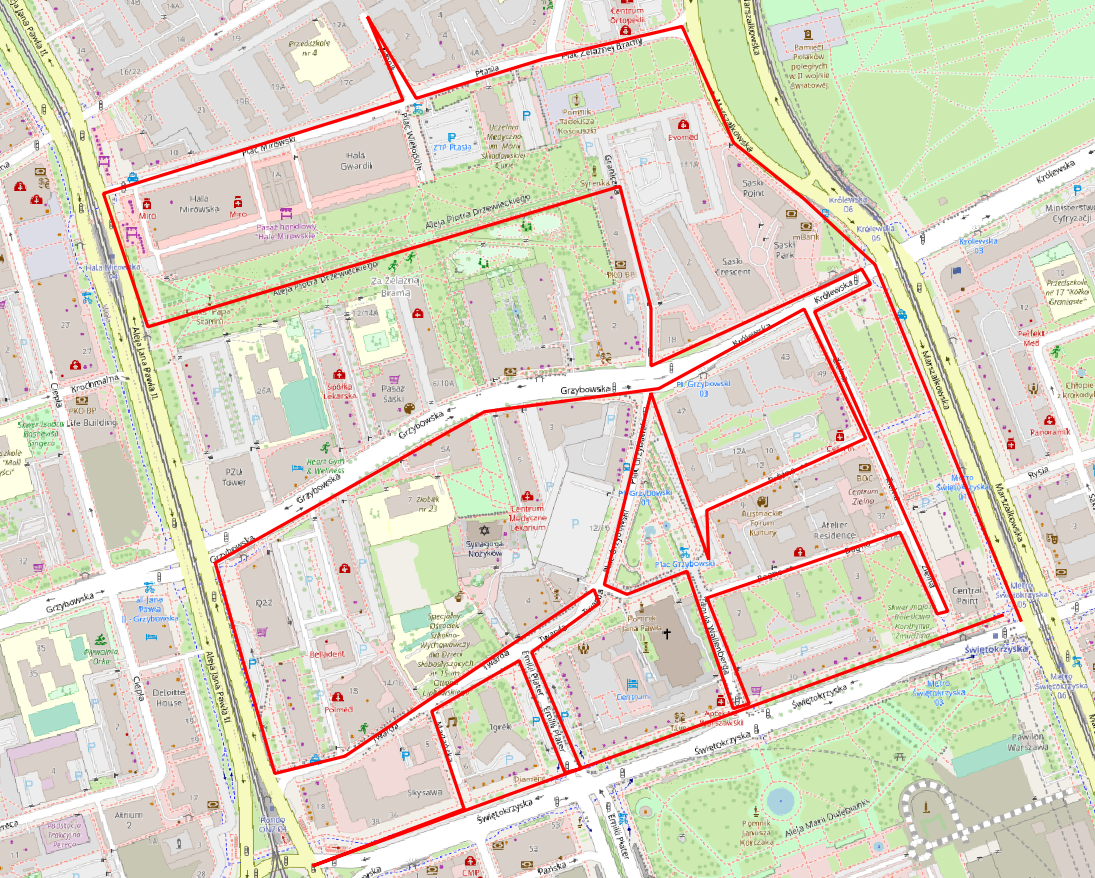
\includegraphics[width=1\linewidth]{route_p10}
			\caption{Planned route}
			\label{fig:a10}
		\end{subfigure}%
		\linebreak
		\begin{subfigure}{.90\textwidth}
			\centering
			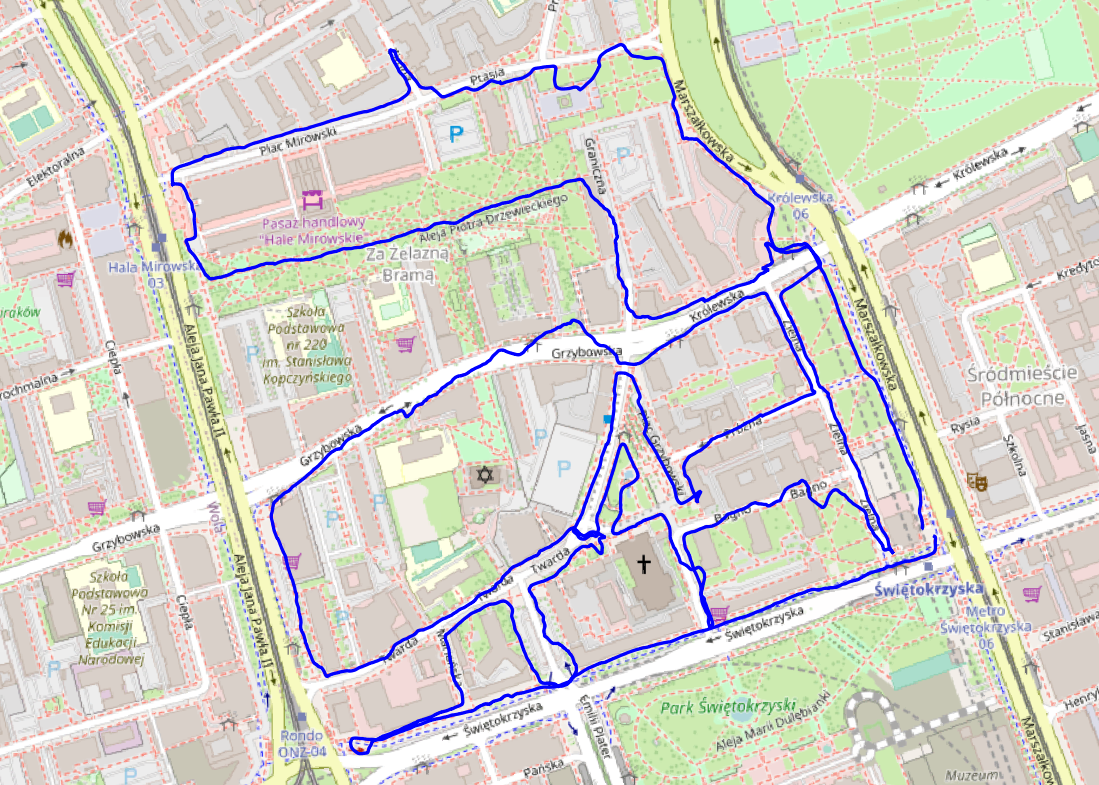
\includegraphics[width=1\linewidth]{route_c10}
			\caption{Covered route}
			\label{fig:b10}
		\end{subfigure}
		\caption{Scan 0010 planned and covered routes.}
		\label{fig:fig10}
	\end{figure} 
	\item \textbf{29.09.2023} Scan 0011. \\
	This scan wasn't complicated nor long, it surrounded a scanning area for 2 October and was calculated to 4,62km (Fig. \ref{fig:a11}). Covered route calculated to 4,85km (Fig. \ref{fig:b11})
	\begin{figure}[H]
		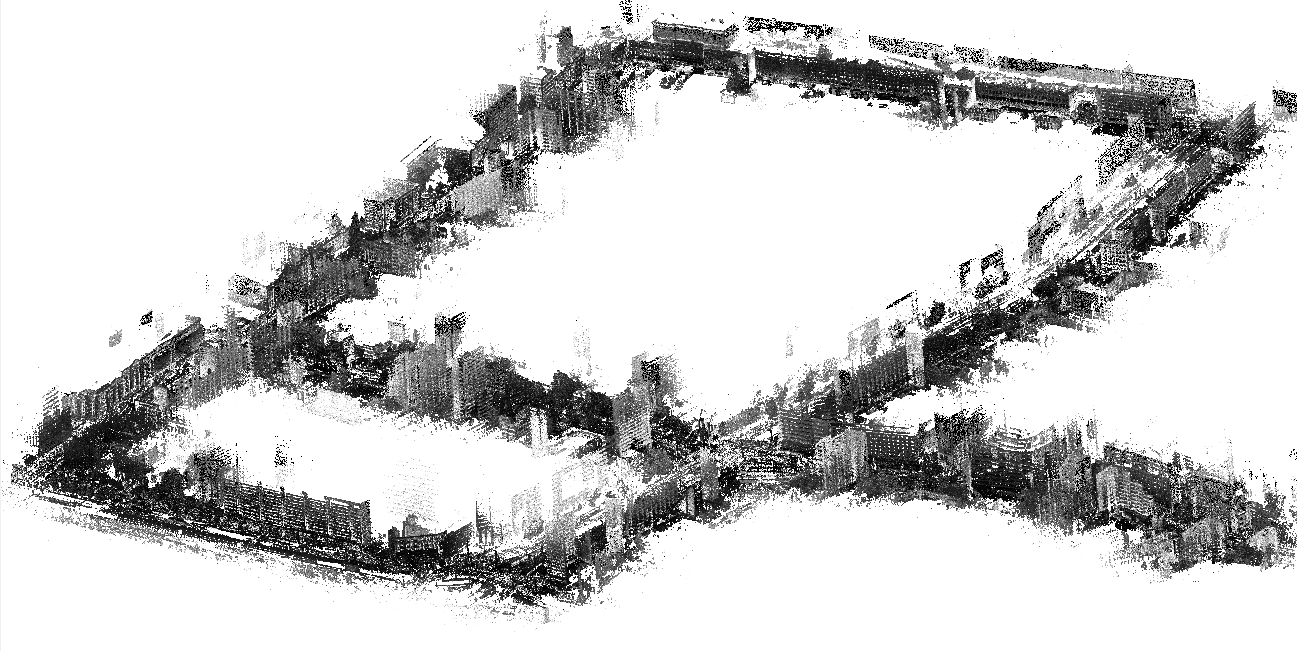
\includegraphics[width=1\linewidth]{cloud11}
		\caption{ContinousScanning\_0011}
	\end{figure}
	\begin{figure}[H]
		\centering
		\begin{subfigure}{.88\textwidth}
			\centering
			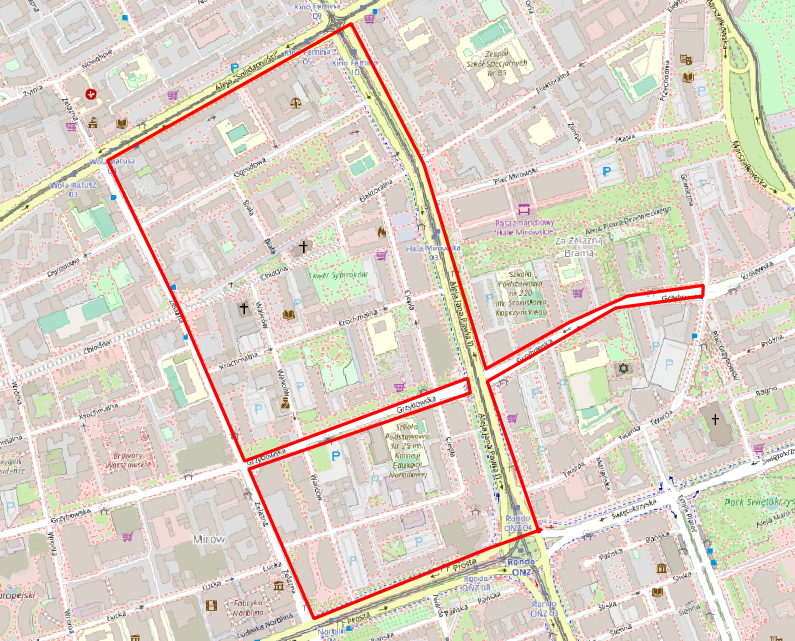
\includegraphics[width=1\linewidth]{route_p11}
			\caption{Planned route}
			\label{fig:a11}
		\end{subfigure}%
		\linebreak
		\begin{subfigure}{.88\textwidth}
			\centering
			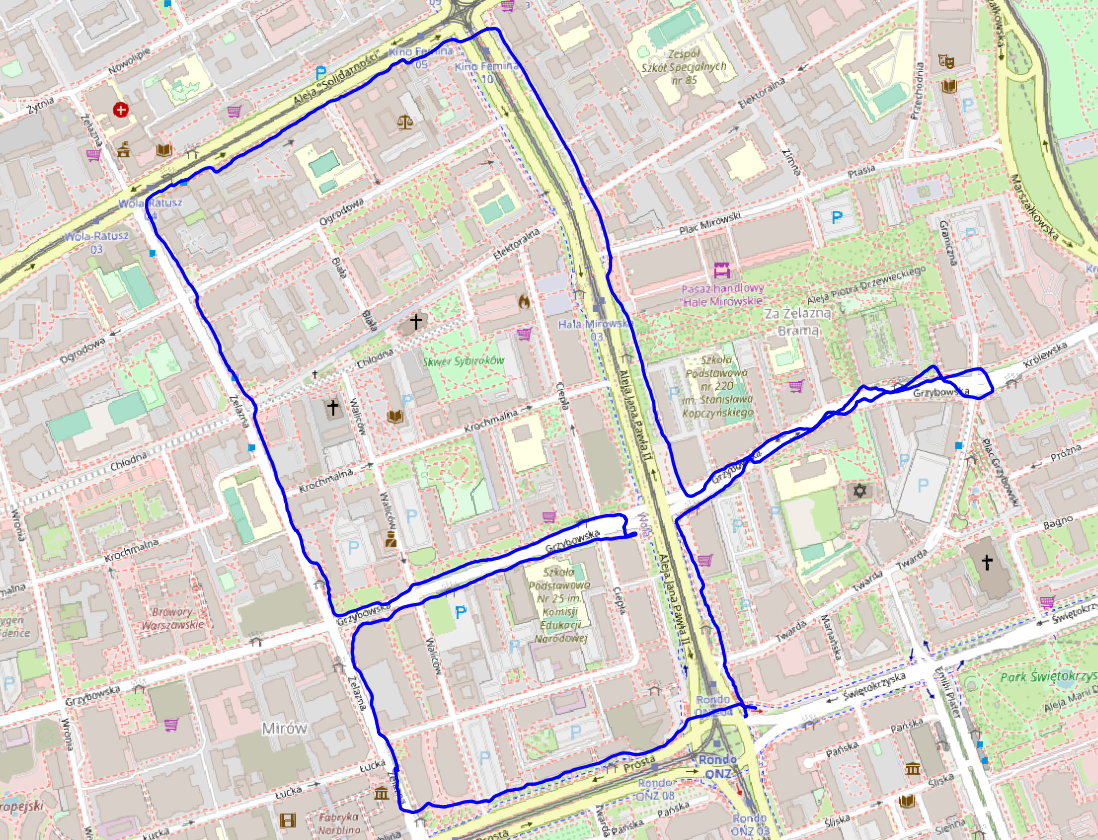
\includegraphics[width=1\linewidth]{route_c11}
			\caption{Covered route}
			\label{fig:b11}
		\end{subfigure}
		\caption{Scan 0011 planned and covered routes.}
		\label{fig:fig11}
	\end{figure} 
\end{enumerate}

\section{Week 2-6 October 2023}
Scans conducted: continousScanning\_0012, continousScanning\_0013, continousScanning\_0014, continousScanning\_0015, continousScanning\_0016.\\
\begin{enumerate}
	\item \textbf{02.10.2023} Scan 0012. \\
	Scanned streets between "Solidarnosci" avenue, Zelazna street, Jana Pawla II avenue and Prosta street. Route according to plan supposed to have 6,23km (Fig. \ref{fig:a12}) and as happened earlier covered route was a little bit longer, because it had 6,65km (Fig. \ref{fig:b12})
	\begin{figure}[H]
		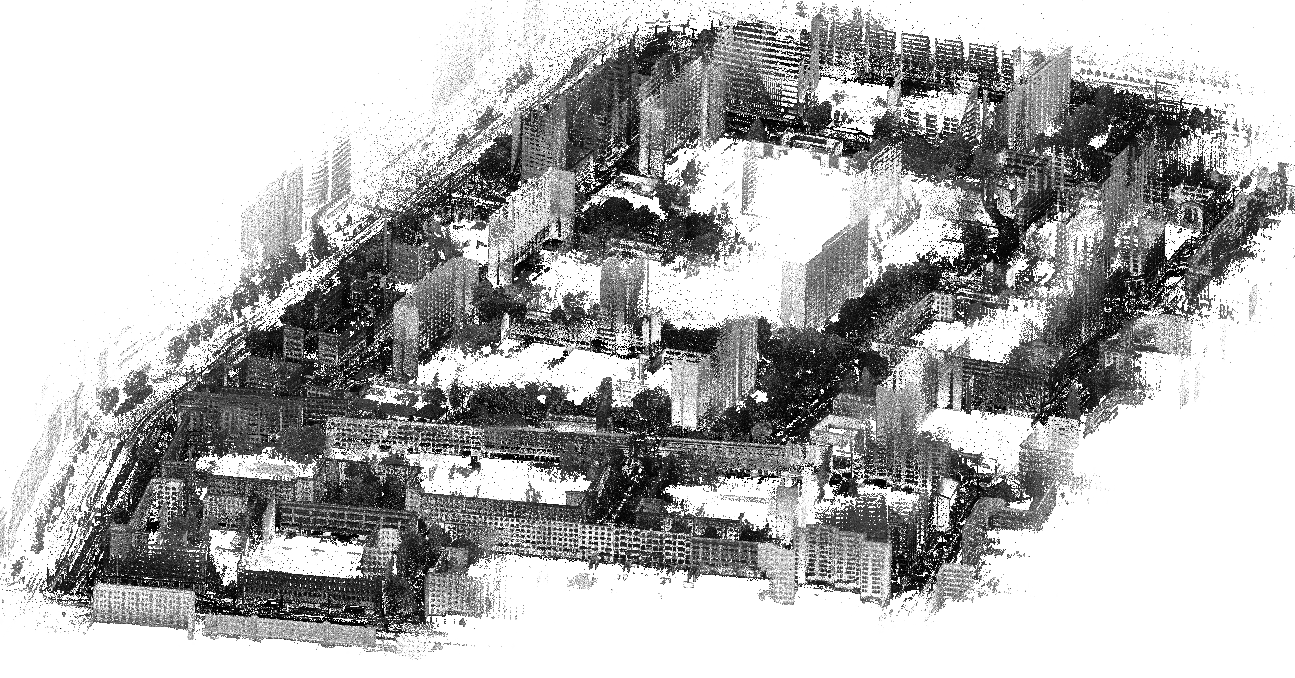
\includegraphics[width=1\linewidth]{cloud12}
		\caption{ContinousScanning\_0012}
	\end{figure}
	\begin{figure}[H]
		\centering
		\begin{subfigure}{.77\textwidth}
			\centering
			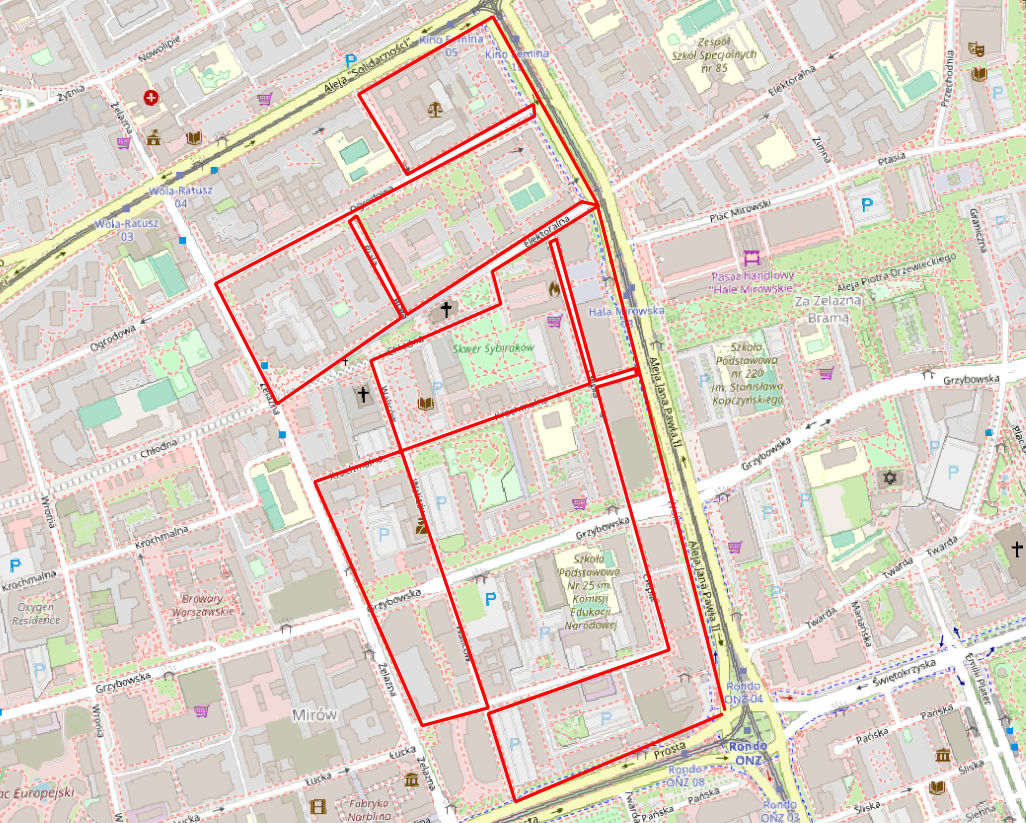
\includegraphics[width=1\linewidth]{route_p12}
			\caption{Planned route}
			\label{fig:a12}
		\end{subfigure}%
		\linebreak
		\begin{subfigure}{.77\textwidth}
			\centering
			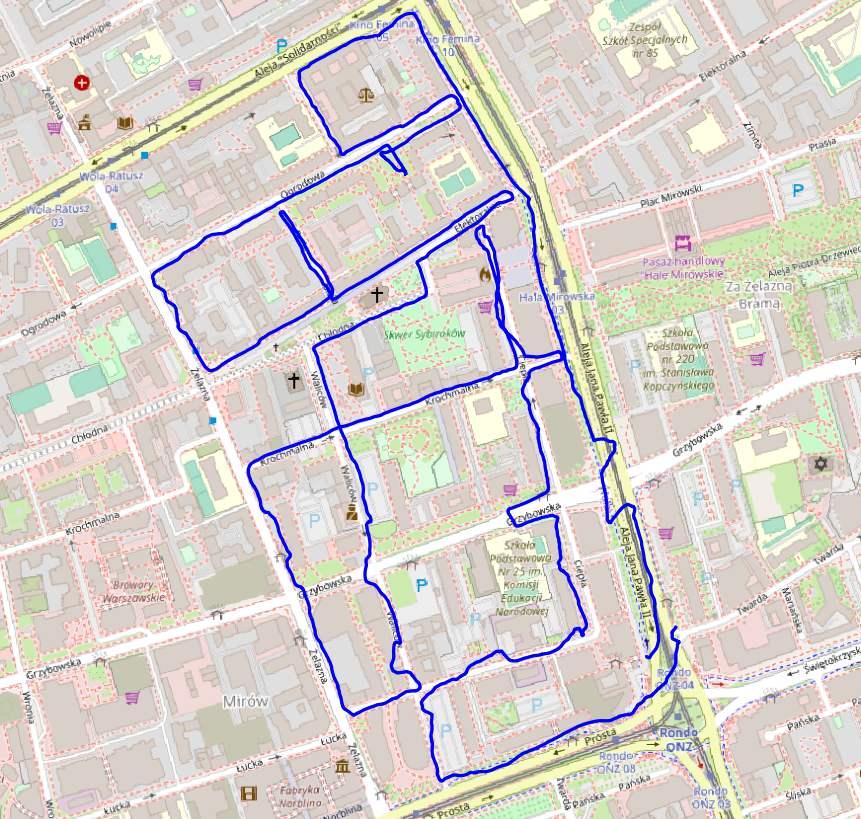
\includegraphics[width=1\linewidth]{route_c12}
			\caption{Covered route}
			\label{fig:b12}
		\end{subfigure}
		\caption{Scan 0012 planned and covered routes.}
		\label{fig:fig12}
	\end{figure} 
	\item \textbf{03.10.2023} Scan 0013. \\
	Route was planned to thoroughly scan Jerozolimskie avenue and create some kind of connector between different point clouds. Planned length was equal to 4,72km (Fig. \ref{fig:a13}), but covered length was longer - 5,45km (Fig. \ref{fig:b13}). This was caused by localizations of pedestrian crossings that weren't as straight as was planned and some detours were needed.
	\begin{figure}[H]
		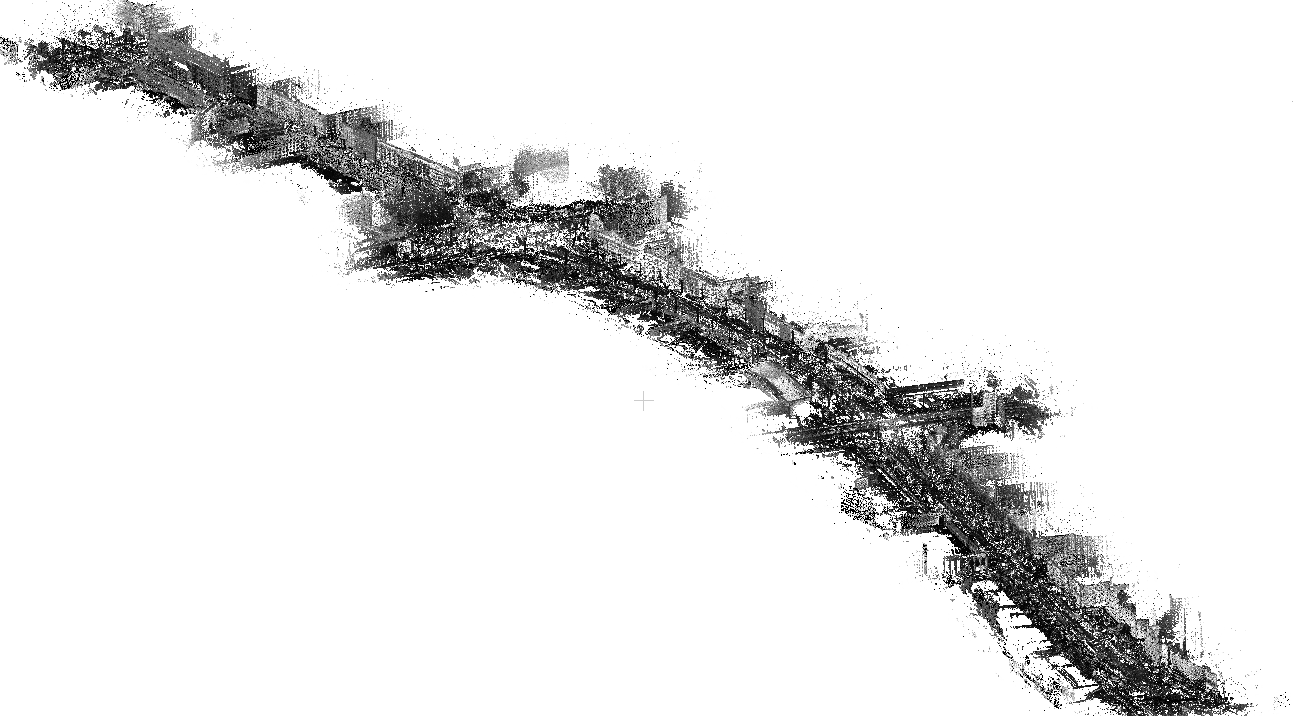
\includegraphics[width=1\linewidth]{cloud13}
		\caption{ContinousScanning\_0013}
	\end{figure}
	\begin{figure}[H]
		\centering
		\begin{subfigure}{.90\textwidth}
			\centering
			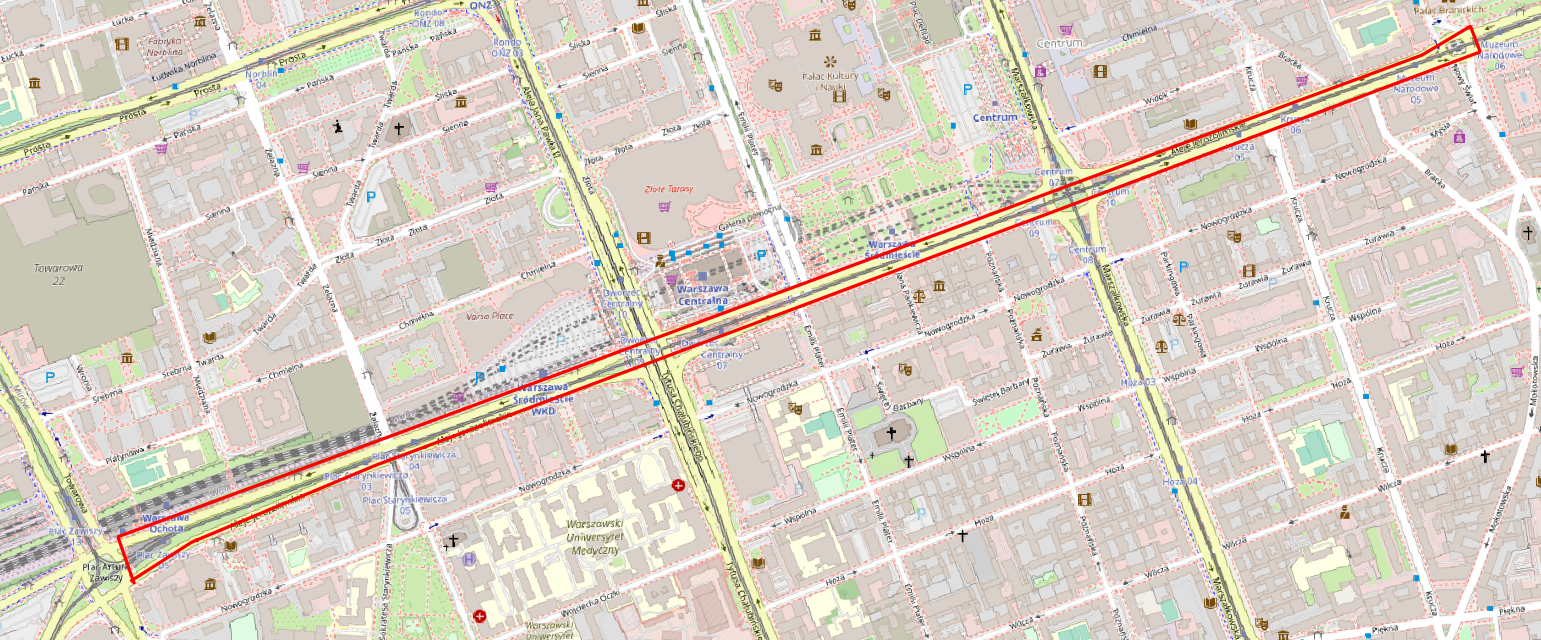
\includegraphics[width=1\linewidth]{route_p13}
			\caption{Planned route}
			\label{fig:a13}
		\end{subfigure}%
		\linebreak
		\begin{subfigure}{.90\textwidth}
			\centering
			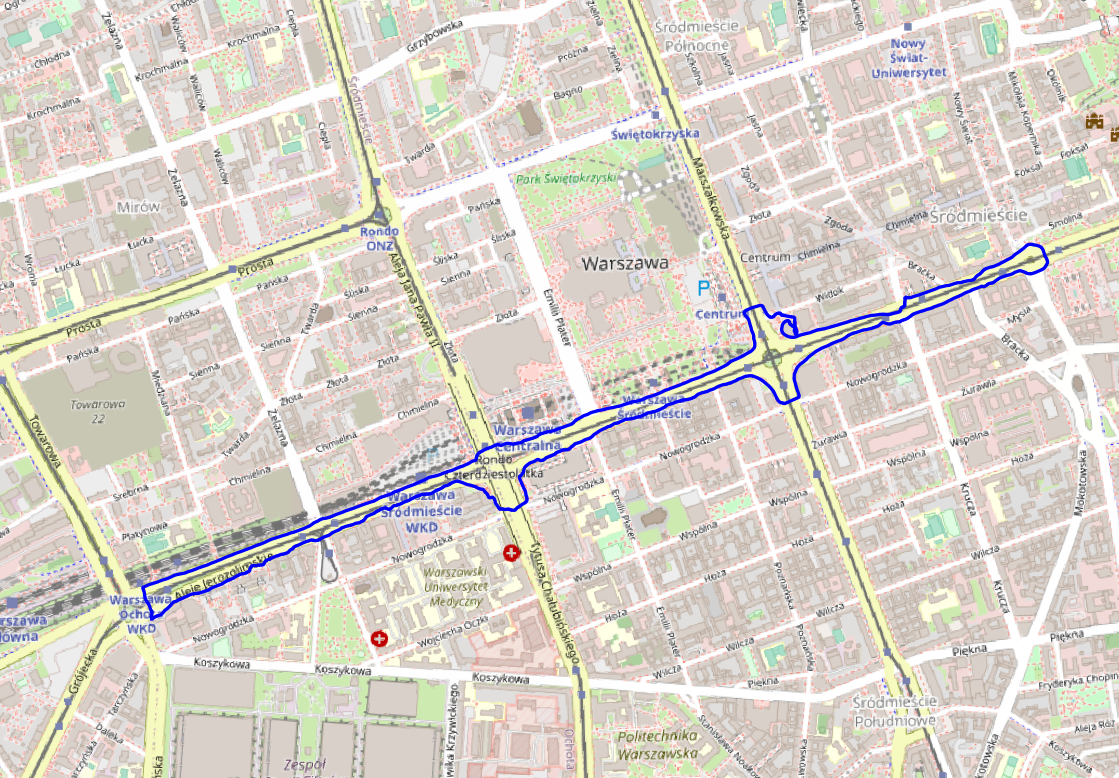
\includegraphics[width=1\linewidth]{route_c13}
			\caption{Covered route}
			\label{fig:b13}
		\end{subfigure}
		\caption{Scan 0013 planned and covered routes.}
		\label{fig:fig13}
	\end{figure}
	\pagebreak
	
	\item \textbf{04.10.2023} Scan 0014. \\
	Streets covered by the scan were all located between Prosta street, Towarowa street, Jerozolimskie avenue and Zelazna street. Planned length of the scanning route was estimated to 5,09km (Fig. \ref{fig:a14}) and covered route reached 5,58km (Fig. \ref{fig:b14}), probably because of additional scanning path near one of the skyscrapers. The path can be seen at the bottom part of Fig. 15b as the difference from Fig. 15a.
	\begin{figure}[H]
		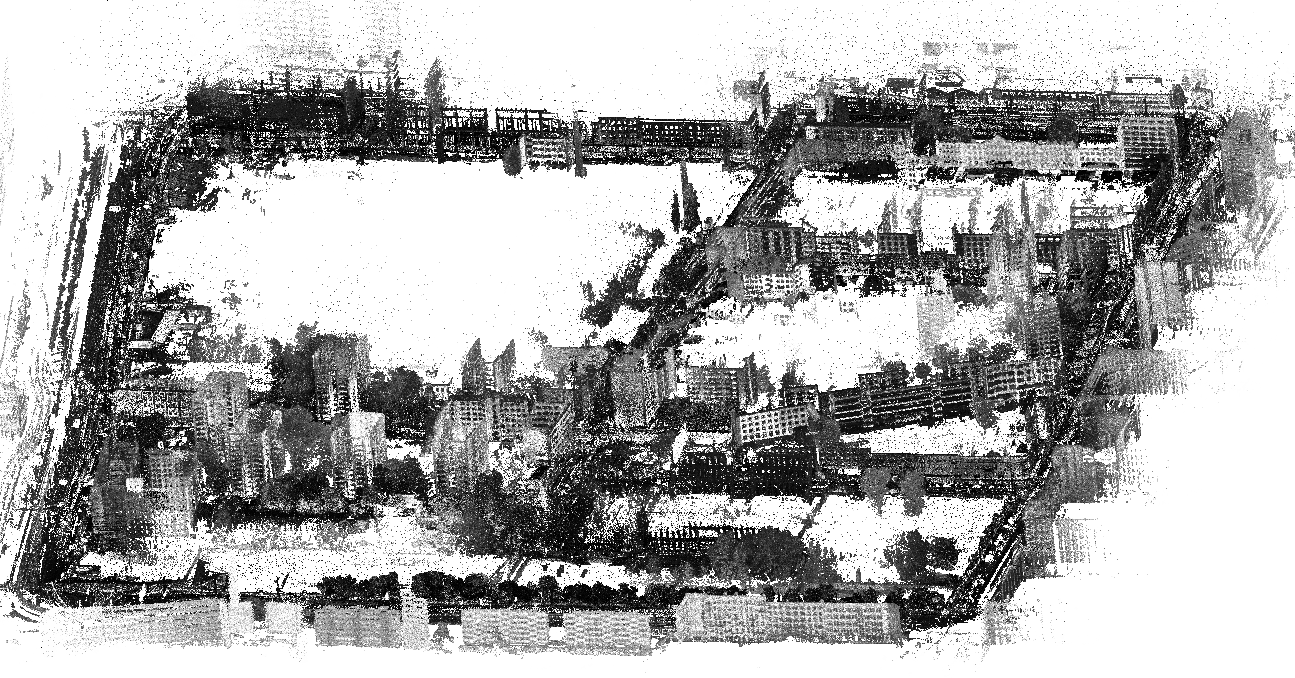
\includegraphics[width=1\linewidth]{cloud14}
		\caption{ContinousScanning\_0014}
	\end{figure}
	\begin{figure}[H]
		\centering
		\begin{subfigure}{.90\textwidth}
			\centering
			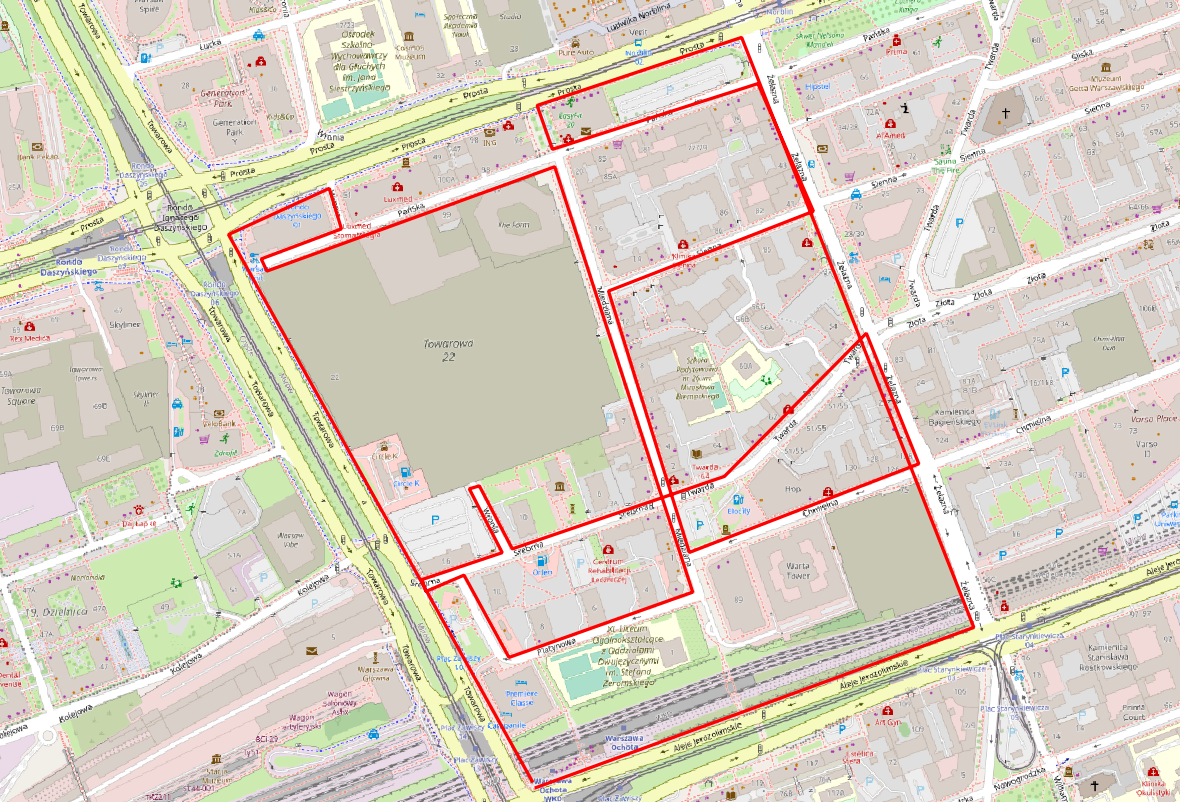
\includegraphics[width=1\linewidth]{route_p14}
			\caption{Planned route}
			\label{fig:a14}
		\end{subfigure}%
		\linebreak
		\begin{subfigure}{.90\textwidth}
			\centering
			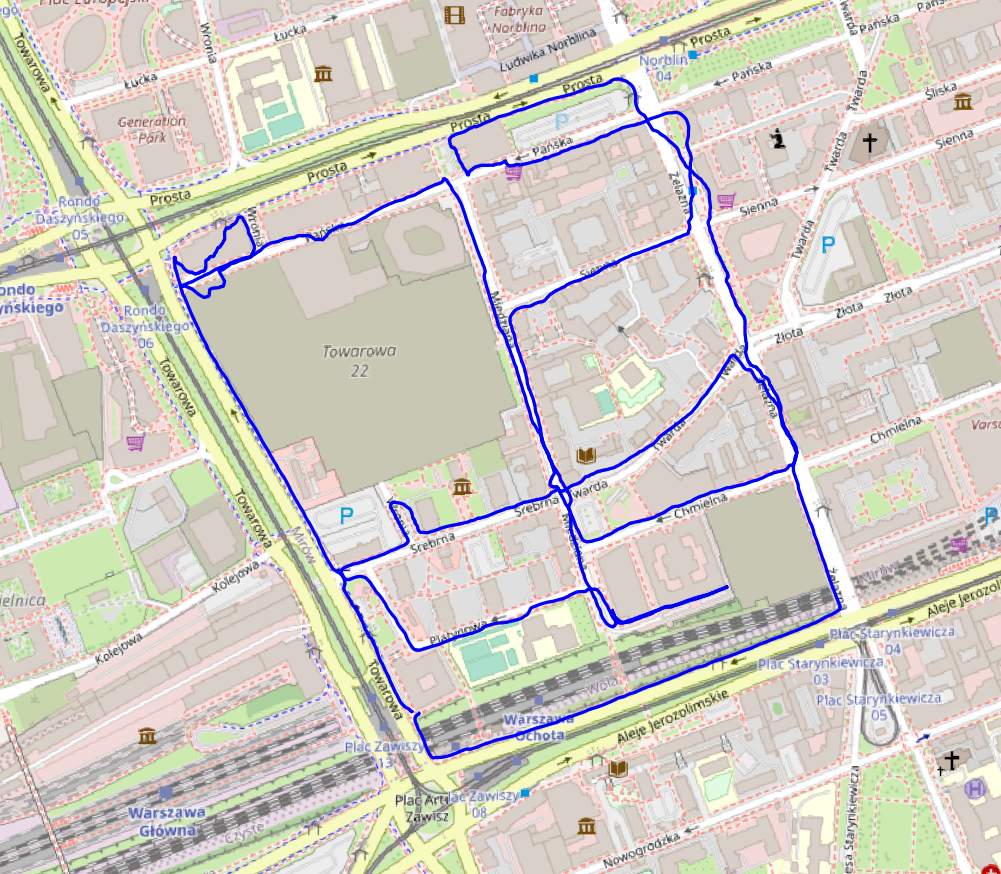
\includegraphics[width=1\linewidth]{route_c14}
			\caption{Covered route}
			\label{fig:b14}
		\end{subfigure}
		\caption{Scan 0014 planned and covered routes.}
		\label{fig:fig14}
	\end{figure} 
	\pagebreak
	
	\item \textbf{05.10.2023} Scan 0015. \\
	Scan was performed north of the previous one, on the opposite site of Prosta street. Planned route length equals 5,07km (Fig. \ref{fig:a15}) and covered one equals 6,3km. Higher covered length is partly caused due to my mistake in the beginning of the scan - i chose wrong path as seen at the bottom of Fig. 16b as it has additional line in comparison to Fig. 16b. The main reason why covered route is longer is that I scanned Krochmalna street (seen at the middle of Fig. \ref{fig:b15}) that wasn't included in the planned routes, since it wasn't added to the database BDOT10k yet, hence the difference.
	\begin{figure}[H]
		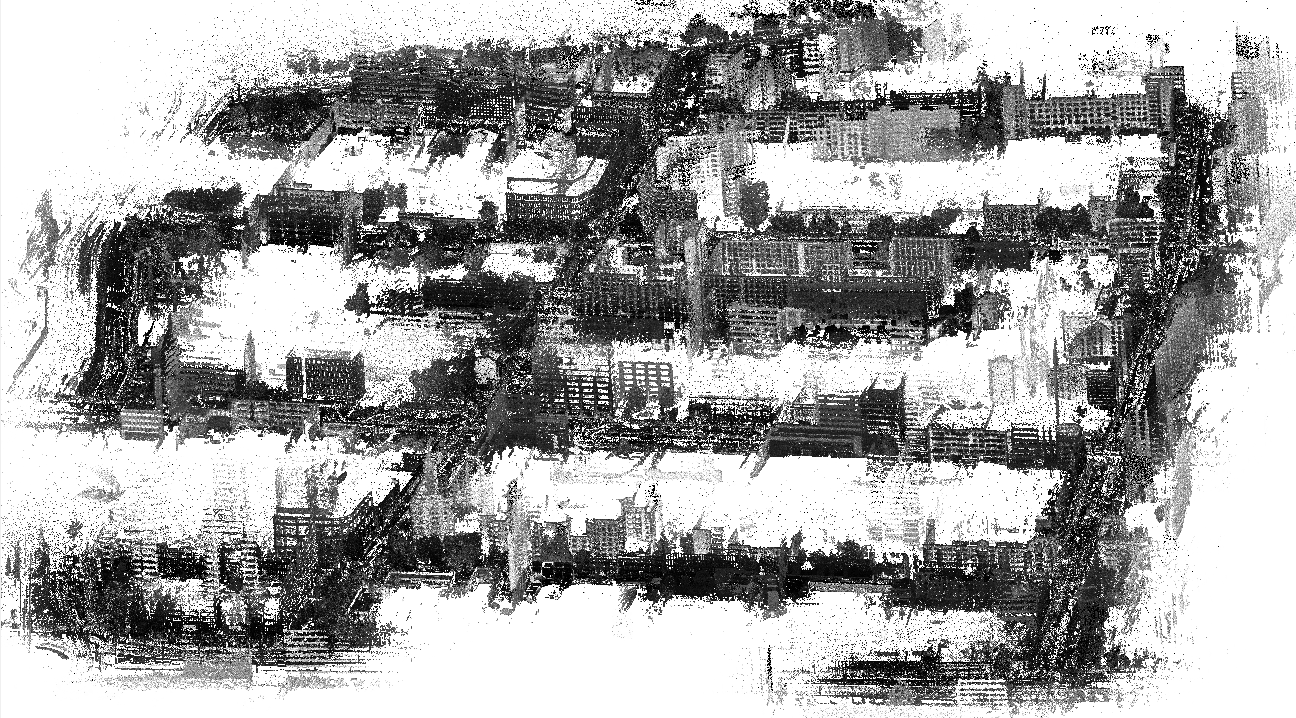
\includegraphics[width=1\linewidth]{cloud15}
		\caption{ContinousScanning\_0015}
	\end{figure} 
	\begin{figure}[H]
		\centering
		\begin{subfigure}{.85\textwidth}
			\centering
			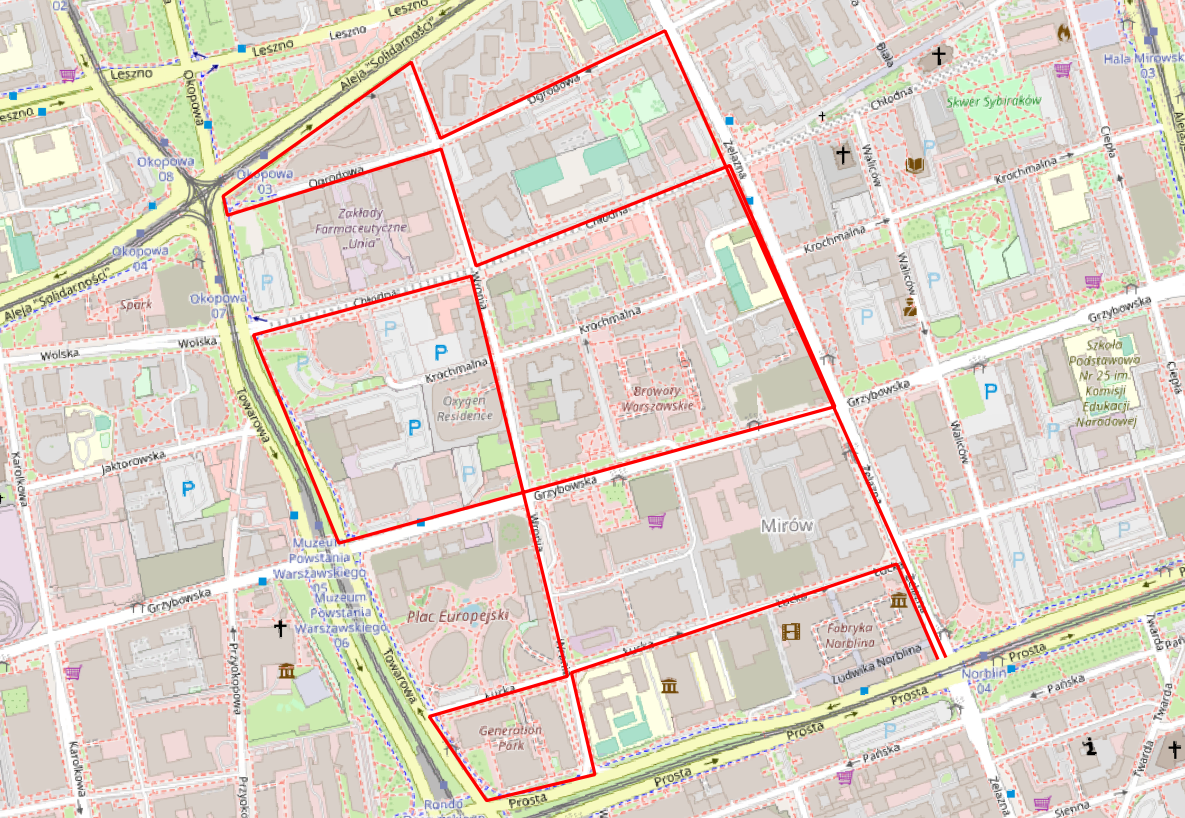
\includegraphics[width=1\linewidth]{route_p15}
			\caption{Planned route}
			\label{fig:a15}
		\end{subfigure}%
		\linebreak
		\begin{subfigure}{.85\textwidth}
			\centering
			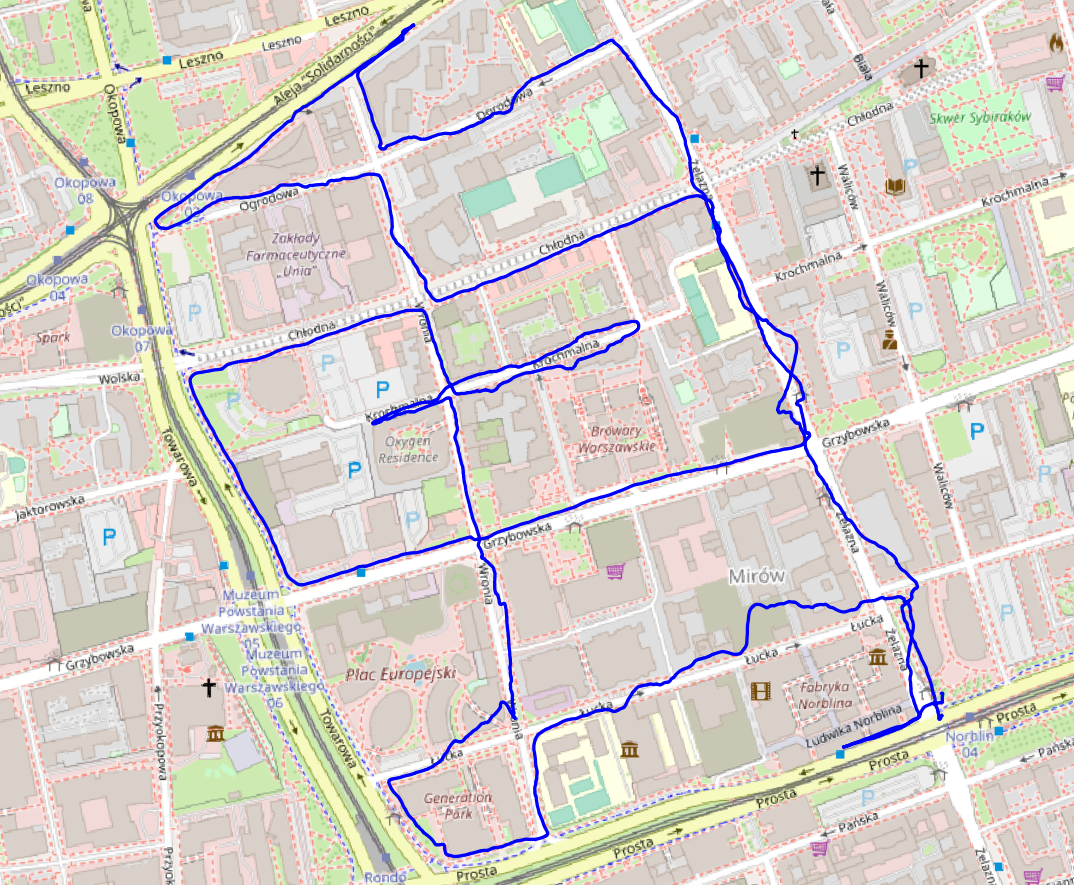
\includegraphics[width=1\linewidth]{route_c15}
			\caption{Covered route}
			\label{fig:b15}
		\end{subfigure}
		\caption{Scan 0015 planned and covered routes.}
		\label{fig:fig15}
	\end{figure} 
	\pagebreak
	
	\item \textbf{06.10.2023} Scan 0016. \\
	Scan route was estimated to 5,50km (Fig. \ref{fig:a16}) and included Raszynska street, Towarowa street, small detour to Grzybowska street and then Solidarnosci avenue. Covered route (Fig. \ref{fig:b16}) appeared to be longer - 6,89km, probably because locations of pedestrian passages and obvious simplification of the planned route. 
	\begin{figure}[H]
		\includegraphics[width=1\linewidth]{cloud16}
		\caption{ContinousScanning\_0016}
	\end{figure}
	\begin{figure}[H]
		\centering
		\begin{subfigure}{.63\textwidth}
			\centering
			\includegraphics[width=1\linewidth]{route_p16}
			\caption{Planned route}
			\label{fig:a16}
		\end{subfigure}%
		\linebreak
		\begin{subfigure}{.63\textwidth}
			\centering
			\includegraphics[width=1\linewidth]{route_c16}
			\caption{Covered route}
			\label{fig:b16}
		\end{subfigure}
		\caption{Scan 0016 planned and covered routes.}
		\label{fig:fig16}
	\end{figure} 
\end{enumerate}

\section{Week 9-13 October 2023}
Scans conducted: continousScanning\_0017.\\
\begin{enumerate}
	\item \textbf{09.10.2023} Scan 0017. \\
	Only one scan caused by my absence in the country from 10th to 16th October. Planned route (Fig. \ref{fig:a17}) length estimated to be 5,60km, but covered route (Fig. \ref{fig:b17}) as happened earlier appeared to be longer and reached 7,06km. Such difference can be explained by assumption made during planning, that there is possibility to walk along Marszalkowska street on the eastern side (the one with Saxon Garden). In reality there was no such possibility resulting in additional distance. Moreover there appeared differences in walking routes along Nowy Przejazd street and lastly my personal endeavours to thoroughly scan Theatre Square as a result adding a few hundred meters.
	\begin{figure}[H]
		\includegraphics[width=1\linewidth]{cloud17}
		\caption{ContinousScanning\_0017}
	\end{figure}
	\begin{figure}[H]
		\centering
		\begin{subfigure}{.75\textwidth}
			\centering
			\includegraphics[width=1\linewidth]{route_p17}
			\caption{Planned route}
			\label{fig:a17}
		\end{subfigure}%
		\linebreak
		\begin{subfigure}{.75\textwidth}
			\centering
			\includegraphics[width=1\linewidth]{route_c17}
			\caption{Covered route}
			\label{fig:b17}
		\end{subfigure}
		\caption{Scan 0017 planned and covered routes.}
		\label{fig:fig17}
	\end{figure} 
\end{enumerate}
\section{Week 16-20 October 2023}
Scans conducted: continousScanning\_0018, continousScanning\_0019, continousScanning\_0020, continousScanning\_0021.\\
\begin{enumerate}
	\item \textbf{17.10.2023} Scan 0018. \\
	First scan conducted after my break, included neighbourhood of Pilsudski Square, and fragments of Senatorska street, Krolewska street and Wierzbowa street. Route was planned to have 4,80km (Fig. \ref{fig:a18}), but covered route (Fig. \ref{fig:b18}) ultimately had 5,47km. Main reason for the difference are construction and excavation works conducted on Piłsudski Square which blocked access to some areas. Worth noting is also my extended scanning of the square which may have had also an impact in longer covered route.
	\begin{figure}[H]
		\includegraphics[width=1\linewidth]{cloud18}
		\caption{ContinousScanning\_0018}
	\end{figure}
	\begin{figure}[H]
		\centering
		\begin{subfigure}{.95\textwidth}
			\centering
			\includegraphics[width=1\linewidth]{route_p18}
			\caption{Planned route}
			\label{fig:a18}
		\end{subfigure}%
		\linebreak
		\begin{subfigure}{.95\textwidth}
			\centering
			\includegraphics[width=1\linewidth]{route_c18}
			\caption{Covered route}
			\label{fig:b18}
		\end{subfigure}
		\caption{Scan 0018 planned and covered routes.}
		\label{fig:fig18}
	\end{figure}
	\item \textbf{18.10.2023} Scan 0019. \\
	Short scan that included "Solidarności" avenue, Jana Pawła II avenue, Elektoralna street, Orla street, Bank Square, Przechodnia and Ptasia street. Planned length of the route (Fig. \ref{fig:a19}) was calculated to 4,56km. Covered route (Fig. \ref{fig:b19}) length was 5,05km long, probably due to minimal changes of the path and/or errors of localization.
	\begin{figure}[H]
		\includegraphics[width=1\linewidth]{cloud19}
		\caption{ContinousScanning\_0019}
	\end{figure}
	\pagebreak
	\begin{figure}[H]
		\centering
		\begin{subfigure}{.95\textwidth}
			\centering
			\includegraphics[width=1\linewidth]{route_p19}
			\caption{Planned route}
			\label{fig:a19}
		\end{subfigure}%
		\linebreak
		\begin{subfigure}{.95\textwidth}
			\centering
			\includegraphics[width=1\linewidth]{route_c19}
			\caption{Covered route}
			\label{fig:b19}
		\end{subfigure}
		\caption{Scan 0019 planned and covered routes.}
		\label{fig:fig19}
	\end{figure} 
	\pagebreak
	\item \textbf{19.10.2023} Scan 0020. \\ 
	Scan was mostly oriented around Savior Square, with paths reaching to Constitution Square, Politechnika Square, Armii Ludowej avenue and Piekna street. Planned route (Fig. \ref{fig:a20}) was calculated to be 5,34km long and the covered route (Fig. \ref{fig:b20}) ended being 5,54km long.
	\begin{figure}[H]
		\includegraphics[width=1\linewidth]{cloud20}
		\caption{ContinousScanning\_0020}
	\end{figure}
	\begin{figure}[H]
		\centering
		\begin{subfigure}{.69\textwidth}
			\centering
			\includegraphics[width=1\linewidth]{route_p20}
			\caption{Planned route}
			\label{fig:a20}
		\end{subfigure}%
		\linebreak
		\begin{subfigure}{.69\textwidth}
			\centering
			\includegraphics[width=1\linewidth]{route_c20}
			\caption{Covered route}
			\label{fig:b20}
		\end{subfigure}
		\caption{Scan 0020 planned and covered routes.}
		\label{fig:fig20}
	\end{figure}
	\item \textbf{20.10.2023} Scan 0021. \\
	A scan started on a crossroad of Koszykowa street and Niepodległości avenue and focused on an area south of that point to Armii Ludowej avenue with a suplementary scan of Nowowiejska street. Planned length (Fig. \ref{fig:a21}) was around 5,54km and covered length summed up to 6,15km (Fig. \ref{fig:b21}), mostly because of my mistakes during scanning, which resulted in a few backtracks. 
	\begin{figure}[H]
		\includegraphics[width=1\linewidth]{cloud21}
		\caption{ContinousScanning\_0021}
	\end{figure}
	\begin{figure}[H]
		\centering
		\begin{subfigure}{.90\textwidth}
			\centering
			\includegraphics[width=1\linewidth]{route_p21}
			\caption{Planned route}
			\label{fig:a21}
		\end{subfigure}%
		\linebreak
		\begin{subfigure}{.90\textwidth}
			\centering
			\includegraphics[width=1\linewidth]{route_c21}
			\caption{Covered route}
			\label{fig:b21}
		\end{subfigure}
		\caption{Scan 0021 planned and covered routes.}
		\label{fig:fig21}
	\end{figure} 
\end{enumerate}
\section{Week 23-27 October 2023}
Scans conducted: continousScanning\_0022, continousScanning\_0023, continousScanning\_0024, continousScanning\_0025.\\
\begin{enumerate}
	\item \textbf{23.10.2023} Scan 0022. \\
	This scan was conducted between Filtrowa street and Wawelska street, with Mianowskiego street as a border from east and Krzywickiego street from west. Total planned length (Fig. \ref{fig:a22}) was estimated to 4,73km and total covered length (Fig. \ref{fig:b22}) didn't differ much, as it was 4,88km.
	\begin{figure}[H]
		\includegraphics[width=1\linewidth]{cloud22}
		\caption{ContinousScanning\_0022}
	\end{figure}
	\pagebreak
	\begin{figure}[H]
		\centering
		\begin{subfigure}{.90\textwidth}
			\centering
			\includegraphics[width=1\linewidth]{route_p22}
			\caption{Planned route}
			\label{fig:a22}
		\end{subfigure}%
		\linebreak
		\begin{subfigure}{.90\textwidth}
			\centering
			\includegraphics[width=1\linewidth]{route_c22}
			\caption{Covered route}
			\label{fig:b22}
		\end{subfigure}
		\caption{Scan 0022 planned and covered routes.}
		\label{fig:fig22}
	\end{figure}
	\pagebreak
	\item \textbf{24.10.2023} Scan 0023. \\
	 Another scan that serves as a "connector" for the scans, included Wawelska street which then goes into Armii Ludowej avenue. Start point was on the crossroad with Grójecka street and a turn back on Marszałkowska street. Route was planned to be 5,23km long (Fig. \ref{fig:a23}) , but due to lack of a surface passage through Niepodległości avenue the covered length increased. On my way to Marszałkowska street I decided to take an underground path (because of too big distance to the nearest pedestrian passage) which resulted in lack of GNSS signal and an error which added additional length after a line from telemetry points was created. On the way back (to Grójecka street) I went along a path to the closest pedestrian passage which wasn't that far away, but still added some meters. These decisions resulted in covered route length reaching 6,43km (Fig. \ref{fig:b23}).
	\begin{figure}[H]
		\includegraphics[width=1\linewidth]{cloud23}
		\caption{ContinousScanning\_0023}
	\end{figure}
	\begin{figure}[H]
		\centering
		\begin{subfigure}{.90\textwidth}
			\centering
			\includegraphics[width=1\linewidth]{route_p23}
			\caption{Planned route}
			\label{fig:a23}
		\end{subfigure}%
		\linebreak
		\begin{subfigure}{.90\textwidth}
			\centering
			\includegraphics[width=1\linewidth]{route_c23}
			\caption{Covered route}
			\label{fig:b23}
		\end{subfigure}
		\caption{Scan 0023 planned and covered routes.}
		\label{fig:fig23}
	\end{figure}
	\pagebreak
	\item \textbf{25.10.2023} Scan 0024 postponed on account of rainfall.

	\item \textbf{26.10.2023} Scan 0024 performed the day after it was planned with more favourable weather conditions. It included mostly Nowy Swiat street and Krakowskie Przedmiescie street, with a part of Castle Square and fragments of streets near it. Scan 0024 served as another "connector" which covered one of the most recognizable streets in the whole city. Planned route was estimated to 5,34km (Fig. \ref{fig:a24}) and covered route reached 5,57km (Fig. \ref{fig:b24}).
	\begin{figure}[H]
		\includegraphics[width=1\linewidth]{cloud24}
		\caption{ContinousScanning\_0024}
	\end{figure}
	\begin{figure}[H]
		\centering
		\begin{subfigure}{.80\textwidth}
			\centering
			\includegraphics[width=1\linewidth]{route_p24}
			\caption{Planned route}
			\label{fig:a24}
		\end{subfigure}%
		\linebreak
		\begin{subfigure}{.80\textwidth}
			\centering
			\includegraphics[width=1\linewidth]{route_c24}
			\caption{Covered route}
			\label{fig:b24}
		\end{subfigure}
		\caption{Scan 0024 planned and covered routes.}
		\label{fig:fig24}
	\end{figure}
	\item \textbf{27.10.2023} Scan 0025 took place on Crossroads square and its surroundings, mostly Ujazdowskie avenue, Ujazdowski park, Piekna street and Armii Ludowej avenue. Planned route was calculated to 5,27km (Fig. \ref{fig:a25}) and covered route was equal to 6,4km (\ref{fig:b25}).
	\begin{figure}[H]
		\includegraphics[width=1\linewidth]{cloud25}
		\caption{ContinousScanning\_0025}
	\end{figure}
	\begin{figure}[H]
		\centering
		\begin{subfigure}{.84\textwidth}
			\centering
			\includegraphics[width=1\linewidth]{route_p25}
			\caption{Planned route}
			\label{fig:a25}
		\end{subfigure}%
		\linebreak
		\begin{subfigure}{.84\textwidth}
			\centering
			\includegraphics[width=1\linewidth]{route_c25}
			\caption{Covered route}
			\label{fig:b25}
		\end{subfigure}
		\caption{Scan 0025 planned and covered routes.}
		\label{fig:fig25}
	\end{figure}
\end{enumerate}

\section{Week 30-31 October 1-3 November 2023}
Scans conducted: continousScanning\_0026, continousScanning\_0027, continousScanning\_0028.\\
\begin{enumerate}
	\item \textbf{30.10.2023} Scan 0026 was conducted on schedule and included region west from Nowy Swiat street, most notably Kruczkowskiego street, part of Jerozolimskie avenue and Tamka street. Planned route was estimated to 5,12km (Fig. \ref{fig:a26}) and covered route reached 5,75km (Fig. \ref{fig:b26}).
	\begin{figure}[H]
		\includegraphics[width=1\linewidth]{cloud26}
		\caption{ContinousScanning\_0026}
	\end{figure}
	\begin{figure}[H]
		\centering
		\begin{subfigure}{.95\textwidth}
			\centering
			\includegraphics[width=1\linewidth]{route_p26}
			\caption{Planned route}
			\label{fig:a26}
		\end{subfigure}%
		\linebreak
		\begin{subfigure}{.95\textwidth}
			\centering
			\includegraphics[width=1\linewidth]{route_c26}
			\caption{Covered route}
			\label{fig:b26}
		\end{subfigure}
		\caption{Scan 0026 planned and covered routes.}
		\label{fig:fig26}
	\end{figure}
	\item \textbf{31.10.2023} Postponed due to rainfall.
	
	\item \textbf{02.11.2023} Scan 0027 took place between Krakowskie Przedmiescie street, Wybrzeze Kosciuszkowskie street, Tamka street and Karowa street. It contains big height difference since the route went through old city bulwark. Planned length was calculated to  6,03km (Fig. \ref{a27}) and covered route was slightly longer - 6,42km (Fig. \ref{fig:b27}).
	\begin{figure}[H]
		\includegraphics[width=1\linewidth]{cloud27}
		\caption{ContinousScanning\_0027}
	\end{figure}
	\begin{figure}[H]
		\centering
		\begin{subfigure}{.88\textwidth}
			\centering
			\includegraphics[width=1\linewidth]{route_p27}
			\caption{Planned route}
			\label{fig:a27}
		\end{subfigure}%
		\linebreak
		\begin{subfigure}{.88\textwidth}
			\centering
			\includegraphics[width=1\linewidth]{route_c27}
			\caption{Covered route}
			\label{fig:b27}
		\end{subfigure}
		\caption{Scan 0027 planned and covered routes.}
		\label{fig:fig27}
	\end{figure}
	\item \textbf{03.11.2023} Scan 0028 was aimed to include Vistula coast west of the Old Town, near Copernicus Science Centre and Mermaid of Warsaw. Route was supposed to have 5,49km (Fig. \ref{fig:a28}) but it reached more than 1km more -  6,88km (Fig. \ref{fig:b28}).
	\begin{figure}[H]
		\includegraphics[width=1\linewidth]{cloud28}
		\caption{ContinousScanning\_0028}
	\end{figure}
	\begin{figure}[H]
		\centering
		\begin{subfigure}{.95\textwidth}
			\centering
			\includegraphics[width=1\linewidth]{route_p28}
			\caption{Planned route}
			\label{fig:a28}
		\end{subfigure}%
		\linebreak
		\begin{subfigure}{.95\textwidth}
			\centering
			\includegraphics[width=1\linewidth]{route_c28}
			\caption{Covered route}
			\label{fig:b28}
		\end{subfigure}
		\caption{Scan 0028 planned and covered routes.}
		\label{fig:fig28}
	\end{figure}
\end{enumerate}

\section{Week 6-10 November 2023}
Scans conducted: continousScanning\_0029.\\
\begin{enumerate}
	\item \textbf{06.11.2023} Scan 0029 was the last scan to do and since there was a need for the Old Town to be covered, route was longer than aimed 5km to ensure that the whole area is scanned. Planned route was estimated to 7,06km (Fig. \ref{fig:a29}) and ultimately it reached even more - 7,85km (Fig. \ref{fig:b29}). The scan included the most important parts of Warsaw Old Town (Old Town market, Royal Castle and whole Castle Square).
	\begin{figure}[H]
		\includegraphics[width=1\linewidth]{cloud29}
		\caption{ContinousScanning\_0029}
	\end{figure}
	\begin{figure}[H]
		\centering
		\begin{subfigure}{.95\textwidth}
			\centering
			\includegraphics[width=1\linewidth]{route_p29}
			\caption{Planned route}
			\label{fig:a29}
		\end{subfigure}%
		\linebreak
		\begin{subfigure}{.95\textwidth}
			\centering
			\includegraphics[width=1\linewidth]{route_c29}
			\caption{Covered route}
			\label{fig:b29}
		\end{subfigure}
		\caption{Scan 0029 planned and covered routes.}
		\label{fig:fig29}
	\end{figure}
\end{enumerate}

\end{document}
